% Origen: Secciones/PI - Analizador Multicanal.md
\chapter{Analizador multicanal}
\label{C:mca}

% Figuras de ESTE capítulo + las compartidas. Siempre al principio del archivo.
\graphicspath{{figs/cap1/}{figs/comunes/}}

En este capítulo describimos qué es un analizador multicanal (MCA), para qué se
lo emplea y qué lugar ocupa en la cadena de medición. Presentamos la
distribución diferencial de alturas, que es la salida del instrumento, y las
etapas del procesamiento digital de cada evento: la apertura, el cierre, el
cálculo de los estadísticos y su publicación al histograma. Después repasamos
los efectos que distorsionan la medición y que el sistema tiene que compensar o,
al menos, reportar: el apilamiento, el \emph{amplitude walk} y el tiempo muerto.
Para este último mostramos por qué hace falta conocerlo con precisión: la
corrección de la tasa amplifica cualquier error en el tiempo muerto, y tanto más
cuanto mayor es la tasa. Cerramos con las figuras de mérito con que se
caracteriza un MCA y con la extensión del histograma a dos dimensiones.

%%%%%%%%%%%%%%%%%%%%%%%%%%%%%%%%%%%%%%%%%%%%%%%%%%%%%%%%%%%%%%%%%%%%%%%%%%%%%%%%
\section{Descripción mínima}
\label{S:mca-descripcion-minima}

La creación de esta herramienta fue el objetivo primordial de este proyecto. Un
MCA construye un \textbf{histograma} de uno o más \emph{estadísticos} de los
pulsos electrónicos; los más utilizados son la altura máxima y la carga
(integral). A pesar de su nombre, un multicanal no necesariamente tiene
múltiples canales: el nombre proviene de un detalle de su implementación
histórica, que se describe en la Sec.~\ref{S:mca-origen-nombre}.

En la Fig.~\ref{f:mca-senal} se presenta su funcionamiento sobre una traza
simulada de la señal cuantizada por un conversor analógico-digital (ADC). El
primer eslabón es el disparador, también llamado \emph{trigger}, con
histéresis: cuando la señal supera un umbral de disparo (\codigo{thr}) se abre
una ventana, que se mantiene abierta hasta que la señal cae por debajo de un
umbral de relajación (\codigo{thr}~$-$~\codigo{hyst}). En la figura el primer
umbral se representa con una línea roja rayada y el segundo con una línea roja
punteada; todas las ventanas (en amarillo) empiezan y terminan donde la curva
corta la línea del umbral correspondiente. Los pulsos que no superan el umbral,
como el \#6, no abren ninguna ventana y no producen ninguna cuenta.

\begin{figure}[H]
\centering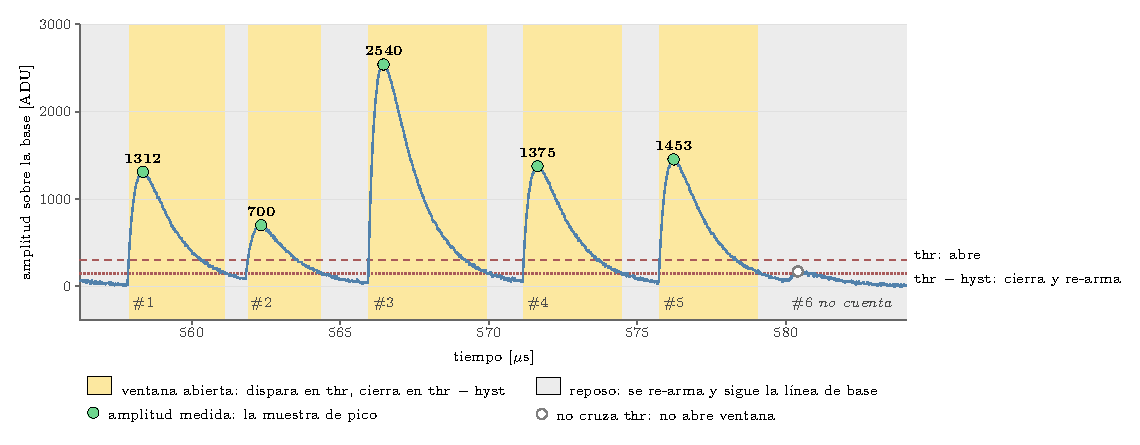
\includegraphics{cap1_senal}
\caption[Funcionamiento esquemático del MCA sobre una traza simulada]{%
Funcionamiento esquemático del MCA sobre una traza simulada con seis pulsos. En
amarillo, la ventana abierta: dispara al cruzar \codigo{thr} y cierra al bajar
de \codigo{thr}~$-$~\codigo{hyst}. En gris, el reposo: el disparador se re-arma
y el seguidor de línea de base actualiza la referencia contra la que se mide la
amplitud. En verde, la amplitud medida de cada pulso.\label{f:mca-senal}}
\end{figure}

Conceptualmente, al cerrarse la ventana tenemos un vector con todas las muestras
del evento, que se transfiere a un extractor de características que calcula
todos los estadísticos en paralelo. En el hardware los estadísticos se calculan
muestra a muestra mientras la ventana está abierta, sin guardar el vector (ver
Sec.~\refpend{S:implmca-recuperacion}{Implementación del MCA: métodos de
recuperación del pulso}). En la Fig.~\ref{f:mca-senal} se presenta únicamente la
altura máxima, con un punto verde en el ápice de cada pulso.

Cada vez que se cierra una ventana, el valor del estadístico se transfiere al
histograma, que suma una cuenta en el canal (o \emph{bin}) correspondiente. A
este mecanismo lo llamamos \emph{publicación} del estimador. En la
Fig.~\ref{f:mca-camino-datos} se presenta este camino de datos: por cada pulso
aceptado viaja un único número, su amplitud, y el histograma suma una cuenta en
el canal \codigo{amp\,\textgreater\textgreater\,6}. El desplazamiento a la
derecha divide la amplitud por $2^6 = 64$, de modo que el rango de 0 a
4095~ADU se agrupa en 64 canales. La tabla inferior lista los pulsos de la
Fig.~\ref{f:mca-senal} tal como los ve el histograma; el \#6 figura como
rechazado porque no superó el umbral. Los detalles del mecanismo de
transferencia de datos para el cálculo del estadístico y su publicación se
presentan en los capítulos de implementación de HW.

\begin{figure}[H]
\centering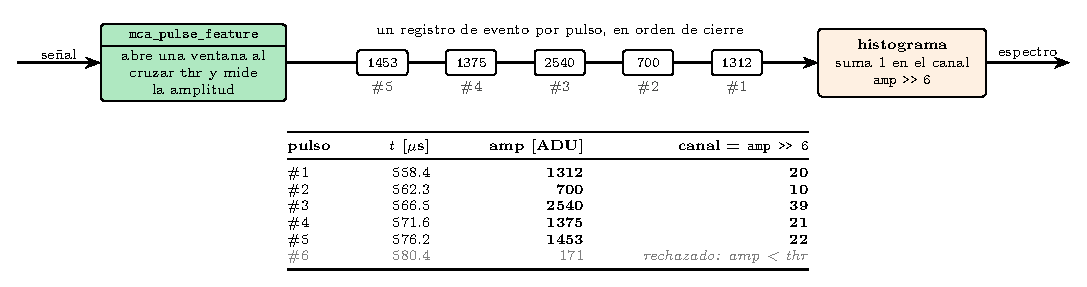
\includegraphics{cap1_camino_datos}
\caption[Camino de datos del MCA]{%
Camino de datos del MCA: un registro de evento por pulso, en orden de cierre, y
la tabla de los pulsos de la Fig.~\ref{f:mca-senal} con su tiempo, su amplitud y
su canal.\label{f:mca-camino-datos}}
\end{figure}

Al acumular las cuentas en un buffer en memoria construimos la
\textbf{distribución diferencial de alturas} ($dN/dH$), que presentamos en la
próxima subsección y que es la salida del módulo. En la
Fig.~\ref{f:mca-histograma} se presenta el espectro final, con la evolución de
la acumulación en barras apiladas: la capa inferior corresponde a las primeras
12 cuentas, la del medio a las cuentas 13 a 64 y la superior a las cuentas 65 a
227. El borde superior de cada capa es el espectro en ese instante. Con las
primeras 12 cuentas no se puede afirmar nada; recién con la acumulación completa
las dos líneas del espectro se distinguen como líneas. A la izquierda del umbral
\codigo{thr} el espectro está vacío por construcción, y no por falta de
estadística.

\begin{figure}[H]
\centering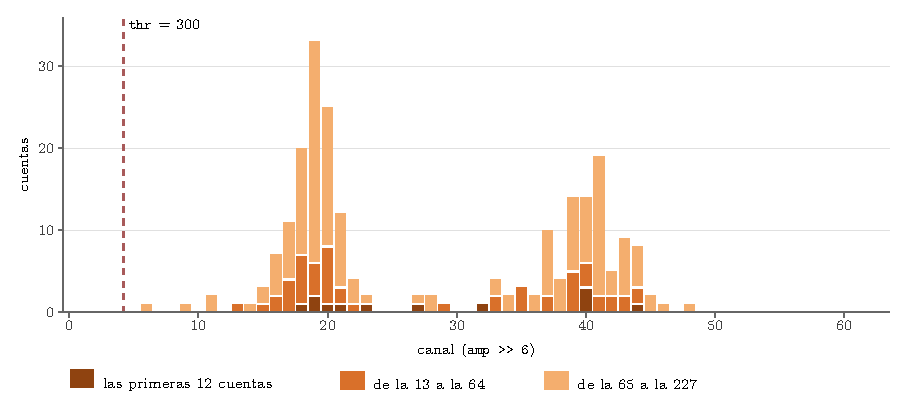
\includegraphics{cap1_histograma}
\caption[Espectro final y evolución de la acumulación]{%
Espectro final en barras apiladas, una capa por tramo de la acumulación: hasta
12, 64 y 227 cuentas. La línea roja marca el umbral \codigo{thr} sobre el eje de
amplitud.\label{f:mca-histograma}}
\end{figure}

Como cada canal es un acumulador, las cuentas del histograma crecen con el
tiempo, a menos que se las reinicie de forma manual.

\subsection{Distribución diferencial de alturas}
\label{S:mca-dda}

La salida del MCA es la \textbf{distribución diferencial de alturas} (DDA), que
escribimos $dN/dH$ (Knoll~\citecap{Knoll2010}{4}). Si $H$ es la altura del pulso
(o el estadístico que se esté histogramando), $dN/dH$ es la cantidad de pulsos
por unidad de altura alrededor de $H$. La cantidad de pulsos con alturas entre
$H_1$ y $H_2$ es su área,
\begin{equation}
  N_{[H_1,\,H_2]} = \int_{H_1}^{H_2} \frac{dN}{dH}\,dH ,
  \label{e:mca-area}
\end{equation}
y el área total, $N_0 = \int_0^{\infty} \frac{dN}{dH}\,dH$, es la cantidad
total de pulsos registrados. En el MCA la altura está discretizada en canales de
ancho $\Delta H$: la integral se vuelve una suma y la cuenta del canal $i$ es
$N_i \simeq \frac{dN}{dH}(H_i)\,\Delta H$. Es una medición de la distribución de
probabilidad de las alturas, sin normalizar: dividiendo por $N_0\,\Delta H$ se
obtiene la densidad de probabilidad.

Su contraparte es la \textbf{distribución integral de alturas} $N(H)$, la
cantidad de pulsos con altura mayor que $H$, que se relaciona con la diferencial
por $dN/dH = -dN(H)/dH$. Es lo que mide un único discriminador con su umbral en
$H$ seguido de un contador, como en la cadena analógica de la
Fig.~\ref{f:mca-cadena-analogica}. No la utilizamos: en la distribución
diferencial las líneas se ven como picos, y su posición, su ancho y su área se
leen de forma directa. Por eso, cuando hablamos del histograma o del espectro
nos referimos siempre a $dN/dH$.

\subsection{Origen histórico del nombre}
\label{S:mca-origen-nombre}

Históricamente, este tipo de análisis empleaba un banco de dispositivos
analógicos llamados \emph{Single Channel Analyzer} (SCA). Cada SCA cuenta los
pulsos cuya altura cae dentro de una ventana fija $[H, H + \Delta H]$,
delimitada por un discriminador inferior y uno superior, de modo que mide un
punto de la distribución diferencial. Cada uno de estos dispositivos se
denominaba canal, y la configuración de múltiples de ellos con ventanas
contiguas, que mide la curva entera de una vez, se llamó \textbf{Multichannel
Analyzer} (MCA). Este esquema se presenta en la Fig.~\ref{f:mca-sca}.

\begin{figure}[H]
\centering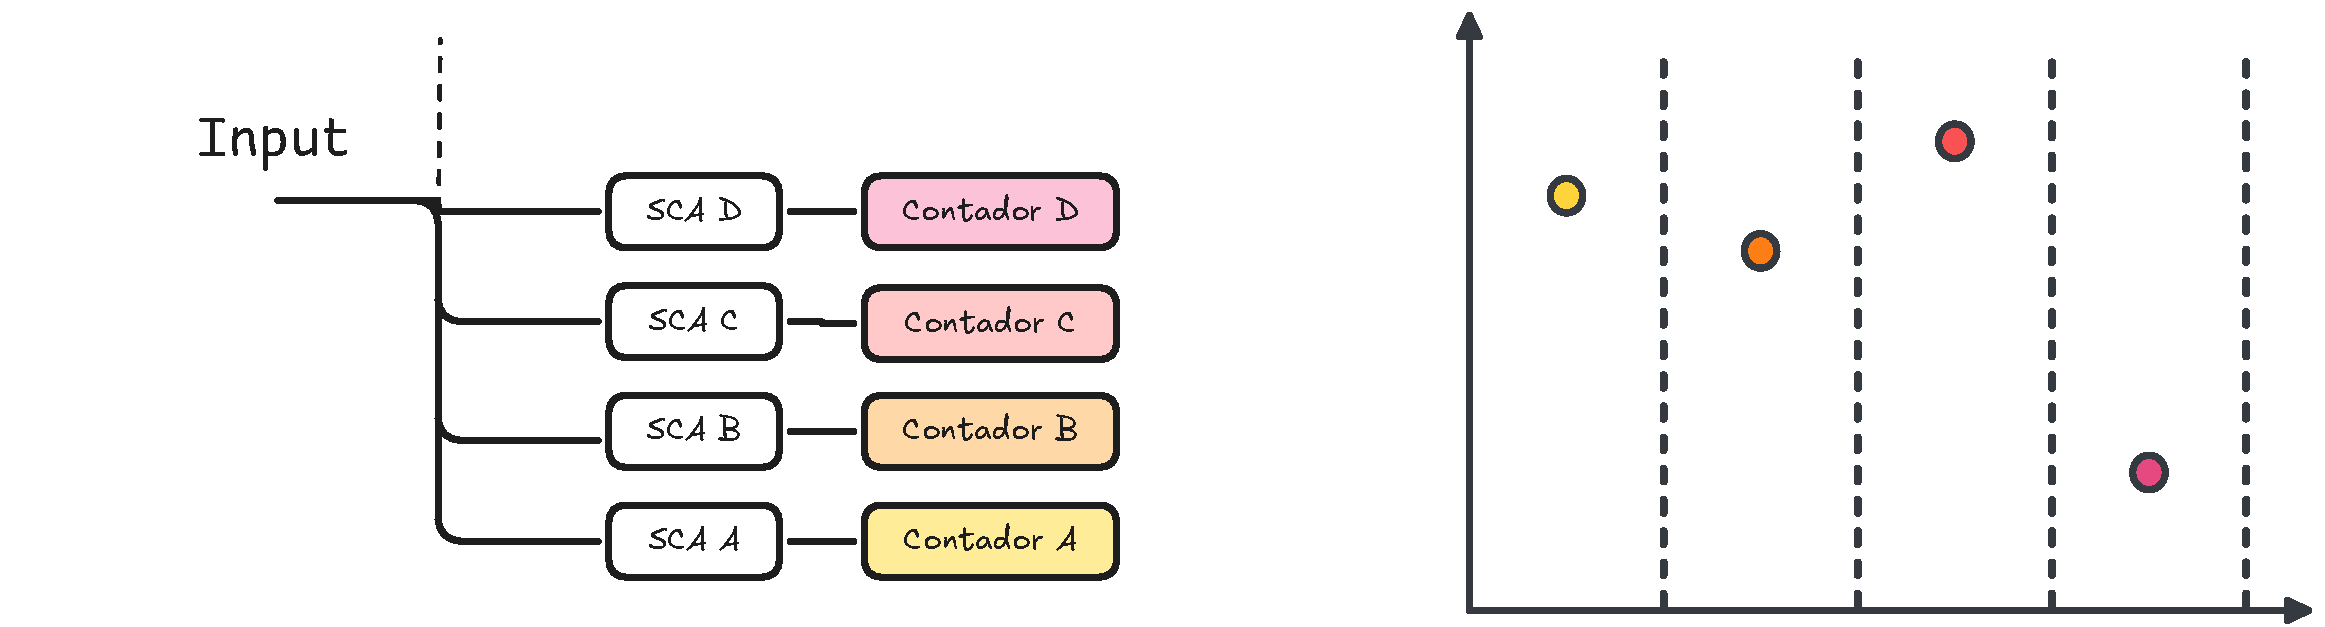
\includegraphics{cap1_sca_mca}
\caption[Un MCA como banco de SCA]{%
Un MCA como banco de SCA: todos reciben la misma entrada y cada uno alimenta a
su propio contador.\label{f:mca-sca}}
\end{figure}

Agregar canales lleva a un muestreo cada vez más fino del espectro continuo,
pero aumenta la varianza relativa de cada canal, porque cada uno recibe menos
cuentas.

En la Fig.~\ref{f:mca-bines} se presentan mediciones con la misma cantidad total
de cuentas del espectro continuo mostrado en (a), variando la cantidad de
canales (o \emph{bines}) utilizados. En (b) la cantidad de canales es demasiado
pequeña para mostrar detalle suficiente; en (c) tenemos la elección que busca un
punto medio entre resolución y fluctuación estadística; y en (d) tenemos tantos
canales que las fluctuaciones estadísticas son tan grandes que podrían
enmascarar picos pequeños. El extremo de pocos canales está acotado por la
corrección de Sheppard~\cite{Sheppard1898}: un canal de ancho $\Delta$ suma
$\Delta^2/12$ a la varianza del pico, y para que no la infle en más de
$\sim$\qty{1}{\percent} hacen falta al menos 4 canales por FWHM. Se detalla en
el Apéndice~\refpend{S:implmca-fisher-bineado}{Poder resolutivo de Fisher en la
elección del bineado}.

\begin{figure}[H]
\centering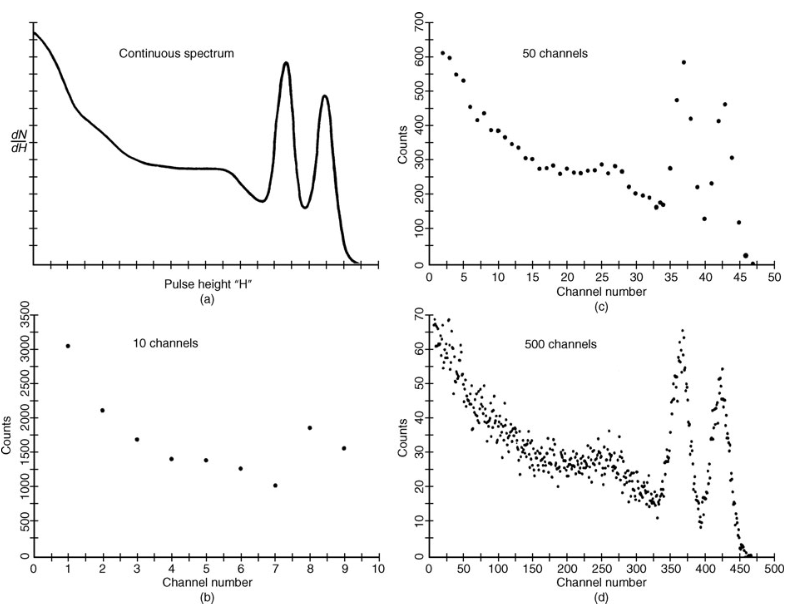
\includegraphics{cap1_bines_knoll}
\caption[Efecto de la cantidad de canales sobre un mismo espectro]{%
Efecto de la cantidad de canales sobre un mismo espectro con igual cantidad
total de cuentas. Extraída de Knoll~\cite[cap.~18, pág.~707]{Knoll2010}.
\label{f:mca-bines}}
\end{figure}

%%%%%%%%%%%%%%%%%%%%%%%%%%%%%%%%%%%%%%%%%%%%%%%%%%%%%%%%%%%%%%%%%%%%%%%%%%%%%%%%
\section{Descripción práctica}
\label{S:mca-descripcion-practica}

En esta sección describimos el \textbf{acercamiento que tiene un nuevo usuario}
frente a este tipo de dispositivos. La idea de este proyecto fue obtener una
versión con el \textbf{mismo conjunto de funcionalidades mínimas} que los
equipos comerciales. Estas funcionalidades deberían incluir al menos:
\begin{itemize}
  \item Capacidad de control de la adquisición: \textbf{reiniciar las cuentas
    presentes} y decidir cuándo \textbf{arrancar y detener la adquisición}.
  \item Capacidad de visualizar el espectro en tiempo real.
  \item \textbf{Guardar} los datos presentes.
  \item Algún sistema de \textbf{advertencia} para indicar \textbf{operación
    fuera de los límites de la especificación} obtenida.
\end{itemize}

En la Fig.~\ref{f:mca-amptek} se presenta una de las interfaces gráficas de
usuario (\emph{Graphical User Interface}, GUI) a las que buscamos acercarnos en
este trabajo. La misma cuenta con:
\begin{itemize}
  \item el espectro, en escala logarítmica y calibrado en energía, con regiones
    de interés (ROI) resaltadas;
  \item la configuración del equipo: cantidad de canales, umbral inferior (LLD),
    tiempo de pico del conformado y ganancia;
  \item el estado de la adquisición: cuentas totales, tasa de entrada, tiempo
    muerto y tiempo de acumulación;
  \item la información del pico seleccionado: centroide, FWHM, área neta con su
    incerteza e identificación de la línea;
  \item la temperatura y la alta tensión del detector.
\end{itemize}

\begin{figure}[H]
\centering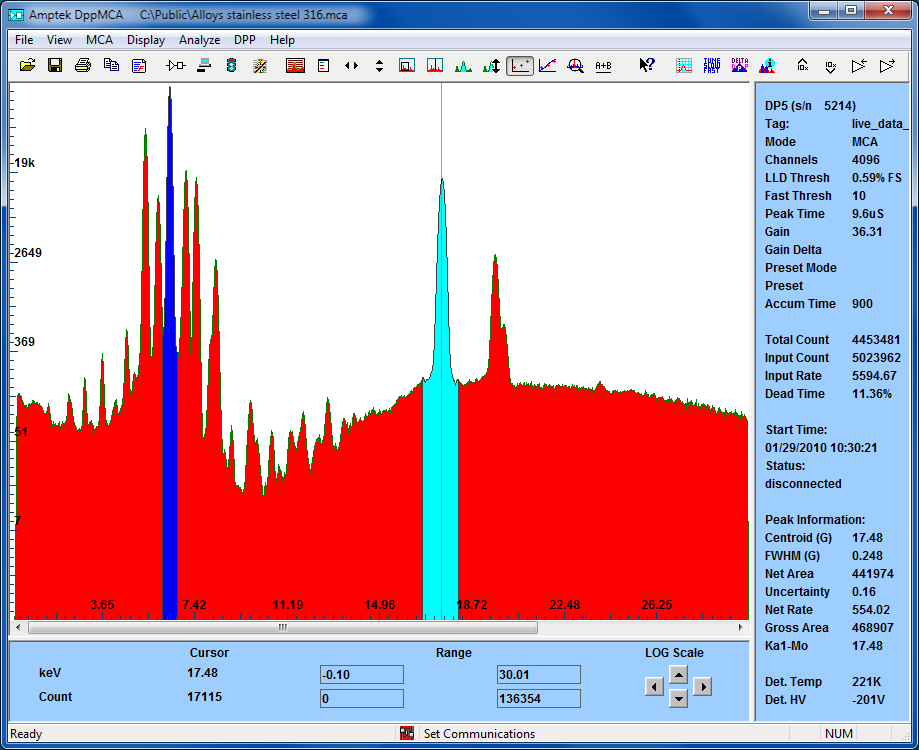
\includegraphics[width=0.6\linewidth]{cap1_amptek_dppmca}
\caption[Software DppMCA del MCA comercial de Amptek]{%
Captura del software propietario que acompaña al MCA comercial de Amptek
(DppMCA)~\cite{AmptekDPPMCA}.\label{f:mca-amptek}}
\end{figure}

La aplicación desarrollada en este trabajo se presenta en la
Sec.~\ref{S:usr-app}.

%%%%%%%%%%%%%%%%%%%%%%%%%%%%%%%%%%%%%%%%%%%%%%%%%%%%%%%%%%%%%%%%%%%%%%%%%%%%%%%%
\section{Cadena de medición típica}
\label{S:mca-cadena-medicion}

El MCA es el \emph{último eslabón} de la cadena de adquisición de un esquema
experimental. Históricamente esta cadena tiene las etapas que se presentan
esquemáticamente en la Fig.~\ref{f:mca-cadena-medicion}:
\begin{enumerate}
  \item \textbf{Detector}:
  \begin{enumerate}
    \item Es el elemento en el que la radiación interactúa y deposita su
      energía. En el Apéndice~\ref{S:ap-detectores} se presenta una tabla con
      las familias de detectores, sus funcionalidades y sus parámetros
      importantes.
    \item El modelo más sencillo lo considera una \textbf{fuente de corriente}:
      cada interacción libera una carga $Q$, proporcional a la energía
      depositada, durante un tiempo de colección que va de nanosegundos a
      microsegundos según el detector. La información de la energía está en la
      carga, $Q = \int i_{sig}(t)\,dt$, y no en la forma del pulso de corriente.
    \item Requiere una \textbf{polarización} (\emph{bias}) de alta tensión, que
      fija la ganancia y el ruido paralelo por corriente de fuga.
  \end{enumerate}
  \item \textbf{Preamplificador}:
  \begin{enumerate}
    \item Su función principal es convertir la \textbf{carga} en
      \textbf{tensión} con la mejor relación señal a ruido (SNR) posible. Por eso
      se lo ubica lo más cerca posible del detector.
    \item Lleva la señal del detector a un rango dinámico en el que las etapas
      siguientes trabajan con mejor precisión.
    \item En la versión sensible a la carga, la salida es un escalón de altura
      $\Delta V = Q/C_F$, con una subida que sigue a la colección de carga y una
      caída exponencial lenta, de constante $R_F C_F$. El tiempo de subida es
      mucho más rápido que el de bajada.
  \end{enumerate}
  \item \textbf{Amplificador de conformado} (\emph{shaping amplifier}):
  \begin{enumerate}
    \item Generalmente contiene una cancelación polo-cero previa, que evita el
      sobreimpulso negativo (\emph{undershoot}) que deja la cola del
      preamplificador al diferenciarla.
    \item Modifica la señal analógica para acortarla, de modo que las colas de
      pulsos sucesivos no se acumulen, y para llevarla a un rango de tensión
      adecuado para las entradas analógicas convencionales.
    \item La elección del filtro fija el \textbf{ancho de banda} del estimador
      de amplitud y, con él, el compromiso entre el ruido serie y el paralelo
      (ver Sec.~\ref{S:mca-tipos-conformado}).
  \end{enumerate}
  \item \textbf{Discriminador o trigger}: decide qué pulsos son eventos. Dispara
    cuando la señal conformada cumple una condición, típicamente superar un
    umbral, y descarta el ruido y los pulsos de baja amplitud. Su salida puede
    ir a un contador, que mide la cantidad de eventos o la tasa, o a un MCA, que
    mide el espectro de energía.
  \item \textbf{Analizador multicanal}:
  \begin{enumerate}
    \item \textbf{Conversión A-D}: transforma la señal analógica mediante una
      cuantización doble. La primera es en tiempo, en la que se suele tener un
      muestreo periódico; la segunda es en valor, para la cual se elige un
      código digital.
    \item \textbf{Restaurador de línea de base}: estima el nivel sobre el que
      monta cada pulso y lo resta, para que la altura medida no dependa de los
      pulsos anteriores ni de derivas lentas.
    \item \textbf{Determinación de eventos}: decide dónde empieza y dónde
      termina cada evento (ver Sec.~\ref{S:mca-etapas}).
    \item \textbf{Cálculo de estadísticos}: calcula la altura, la carga u otros
      estadísticos de cada evento.
    \item \textbf{Discriminador}: decide si el evento entra o no al histograma,
      comparando uno de sus estadísticos contra un intervalo.
    \item \textbf{Contador (histograma)}: suma una cuenta en el canal que
      corresponde al estadístico del evento.
  \end{enumerate}
\end{enumerate}

\begin{figure}[H]
\centering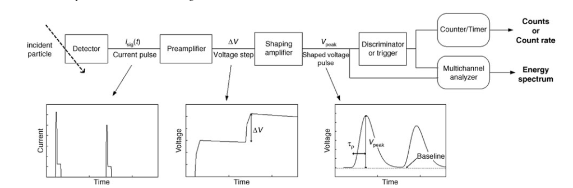
\includegraphics{cap1_cadena_medicion}
\caption[Cadena de medición típica]{%
Cadena de medición típica: detector, preamplificador, amplificador de conformado
y discriminador, seguidos de un contador o de un MCA.\label{f:mca-cadena-medicion}}
\end{figure}

Históricamente, cada una de estas etapas, hasta la discriminación, tenía una
correspondencia directa con un circuito analógico. En la
Fig.~\ref{f:mca-cadena-analogica} se presenta una implementación simple: un
detector de ionización seguido de un preamplificador sensible a la carga, al que
le sigue un amplificador de conformado CR-RC (un pasaaltos, una ganancia y un
pasabajos en cascada) y, a continuación, un detector de eventos por nivel
implementado con un comparador de umbral $V_{LLD}$, cuya salida se lleva a un
contador.

\begin{figure}[H]
\centering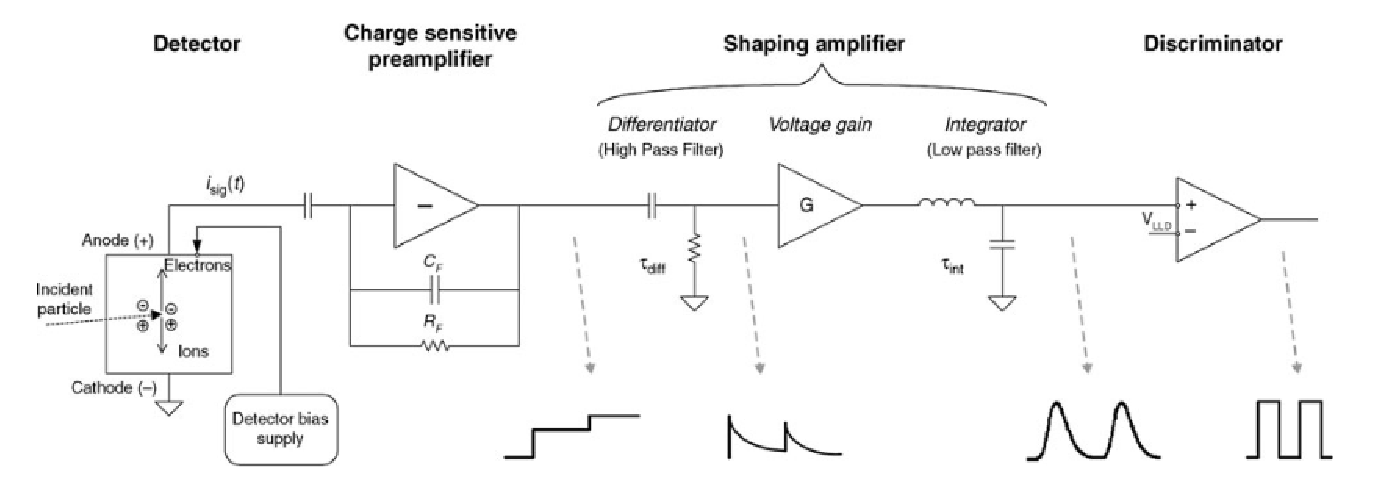
\includegraphics{cap1_cadena_analogica_mca}
\caption[Electrónica simple de procesamiento de señal de un detector]{%
Electrónica simple de procesamiento de señal de un detector. Extraída de
Knoll~\citefig{Knoll2010}{16.2}.\label{f:mca-cadena-analogica}}
\end{figure}

Como el comparador evalúa únicamente la condición $V > V_{LLD}$, las cuentas
resultantes representan la distribución integral de alturas, $N(V_{LLD})$ (ver
Sec.~\ref{S:mca-dda}). Para obtener el espectro hay que barrer el umbral o
reemplazar el comparador por un banco de canales.

En la actualidad, con hardware de tasas de adquisición suficientemente altas en
términos de muestras por pulso (por ejemplo, más de 10), obtenemos un grado de
recuperación digital del pulso que permite emplear técnicas de procesamiento
digital de señales (DSP). Aunque el filtrado de conformado puede implementarse
digitalmente, una etapa analógica previa al ADC sigue siendo necesaria por las
siguientes razones:
\begin{itemize}
  \item \textbf{Rango dinámico y apilamiento}: la señal del preamplificador
    presenta colas exponenciales de decenas de \unit{\micro\second}. A tasas
    altas, estas colas se acumulan (\emph{pileup}) y desplazan la línea de base,
    lo que puede saturar el ADC. La cancelación polo-cero y el acortamiento
    analógico del pulso mantienen la señal acotada. Esto debe hacerse antes de
    digitalizar, porque una saturación no puede corregirse después.
  \item \textbf{Consideraciones de ruido}:
  \begin{enumerate}
    \item \textbf{Antialiasing}: el muestreo exige que la entrada al ADC no
      tenga contenido por encima de $f_s/2$ (teorema de
      Nyquist~\citecap{Oppenheim2010}{4}). El ruido de banda ancha del
      preamplificador que supera ese límite se pliega dentro de la banda útil, y
      ningún filtro digital posterior puede separarlo. Esto requiere un
      pasabajos analógico, aunque no necesariamente un conformador completo.
    \item \textbf{Ruido de digitalización}: el ruido propio del ADC
      (cuantización, ruido térmico) es fijo en LSB y se suma en cuadratura al
      del detector. Una ganancia analógica $G$ previa lo reduce en un factor $G$
      cuando se lo refiere a la entrada, de modo que la resolución queda
      limitada por el ruido del detector y no por el del ADC. La ganancia está
      acotada por el rango dinámico: el pulso máximo, más la excursión de la
      línea de base, no debe saturar el conversor.
  \end{enumerate}
\end{itemize}

De forma que la cadena utilizada en este proyecto se aproxima a la presentada en
la Fig.~\ref{f:mca-cadena-pitaya}: la señal del amplificador de conformado entra
a la Red Pitaya~\cite{RedPitayaDocs} por su entrada analógica (IN), y todos los
elementos posteriores tienen lugar en el dominio digital. Además, el sistema
digital retoma parte del conformado: la cancelación polo-cero y el conformado
trapezoidal digitales~\cite{Jordanov1994} (ver
Sec.~\refpend{S:implmca-trapezoidal}{Implementación del MCA: recuperación por
conformación trapezoidal}).

\begin{figure}[H]
\centering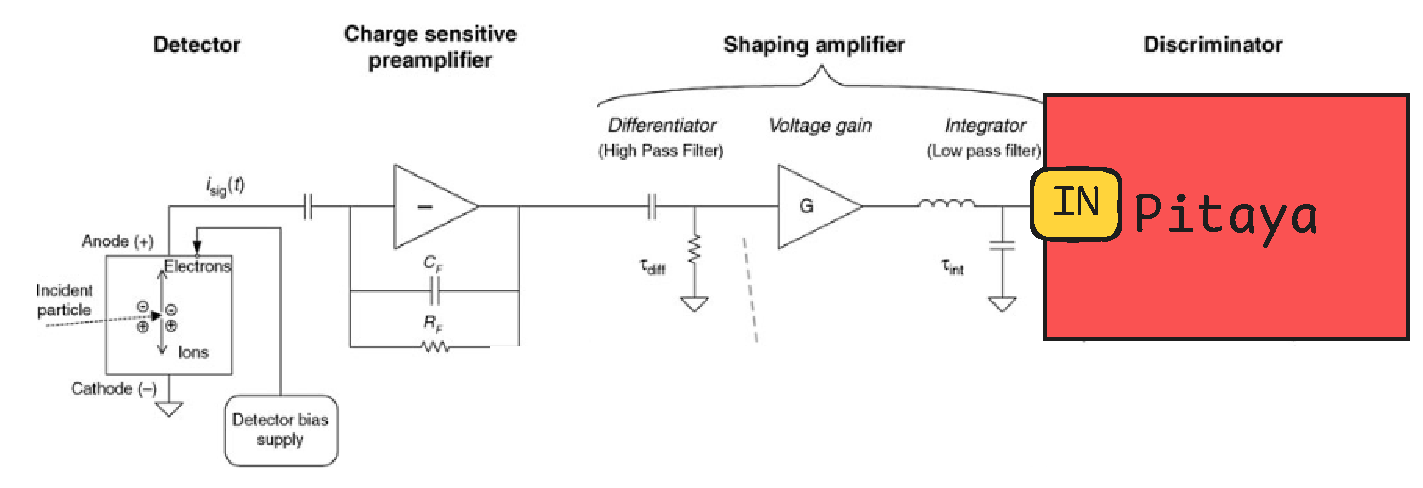
\includegraphics{cap1_cadena_pitaya}
\caption[Cadena de medición utilizada en este trabajo]{%
Cadena utilizada en este trabajo sobre el esquema de la
Fig.~\ref{f:mca-cadena-analogica}: el sistema digital adopta parte de la
conformación de pulsos, la discriminación y el conteo.\label{f:mca-cadena-pitaya}}
\end{figure}

Como este procesamiento previo fija la forma de los pulsos que llegan al MCA, en
la siguiente sección se exploran las diferentes variantes de conformado.

\subsection{Tipos de conformado}
\label{S:mca-tipos-conformado}

En la fase de conformación se aplica algún \textbf{amplificador de conformado}
(Knoll~\citecap{Knoll2010}{16}). En la Fig.~\ref{f:mca-familias} se presentan
las seis familias de conformado de pulsos más aplicadas históricamente,
sintetizadas a partir de su expresión analítica con un ancho a media altura
FWHM~=~\qty{2}{\micro\second} y una altura máxima $A = \qty{0.25}{\volt}$. Son
las formas que usamos como estímulo en las pruebas con el generador de
funciones.

\begin{figure}[H]
\centering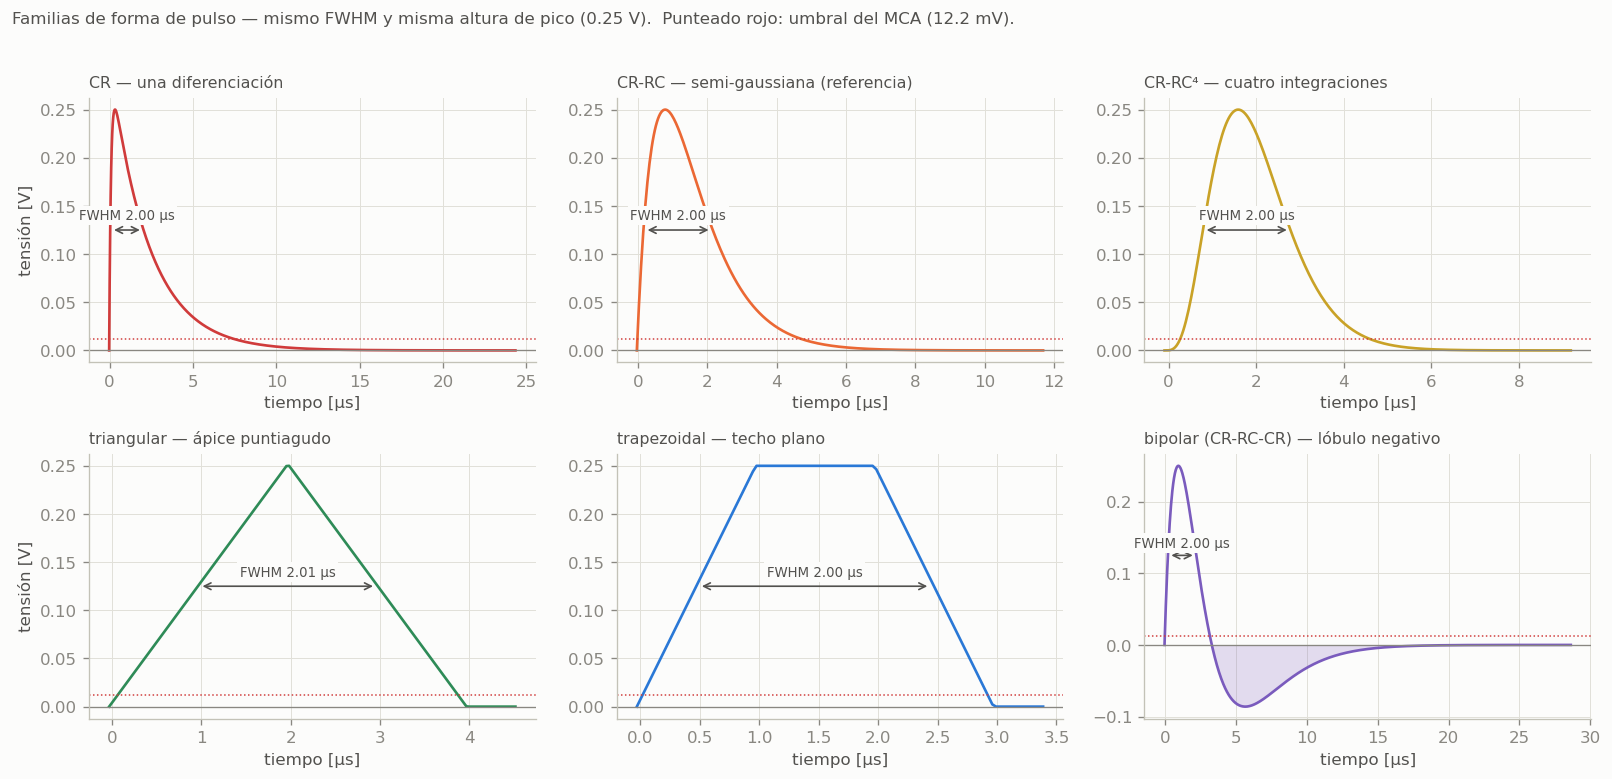
\includegraphics{cap1_familias_conformado}
\caption[Las seis familias de conformado]{%
Las seis familias de conformado, con el mismo FWHM y la misma altura máxima.
\label{f:mca-familias}}
\end{figure}

Estas pueden aproximarse con funciones analíticas $f(u)$, con $u$ el tiempo
normalizado por la constante de tiempo del conformador. Sus características
cualitativas se presentan en la Tabla~\ref{t:mca-conformados}.

\begin{table}[H]
\centering
\caption[Familias de conformado principales]{%
Familias de conformado principales empleadas antes de un MCA.
\label{t:mca-conformados}}
\renewcommand{\arraystretch}{1.6}
\begin{tabular}{|l|l|}
\hline
\encabezado \textbf{Familia} & \textbf{$f(u)$} \\ \hline
\codigo{cr} & $\left(1 - e^{-u/r}\right)e^{-u}$, \ $r = 0.05$ \\ \hline
\codigo{cr\_rc} & $u\,e^{-u}$ \\ \hline
\codigo{cr\_rc4} & $\dfrac{u^{n}e^{-u}}{n!}$, \ $n = 4$ \\ \hline
\codigo{triangular} & $u$ en $[0,1]$; \ $2-u$ en $(1,2]$ \\ \hline
\codigo{trapezoidal} & $u$ en $[0,1]$; \ $1$ en $(1,1{+}p]$; \ $2{+}p-u$ después; \ $p = 1$ \\ \hline
\codigo{bipolar} & $\left(1-\dfrac{u}{2}\right)u\,e^{-u}$ \\ \hline
\end{tabular}
\end{table}

La forma del pulso no es indiferente para el MCA: cada una de las compensaciones
internas se apoya en alguna propiedad de la forma, y la que favorece a una puede
perjudicar a otra.
\begin{itemize}
  \item \textbf{Estimador de altura máxima}: importa cuánto dura el ápice. El
    trapecio mantiene el máximo durante toda su meseta y el ADC lo muestrea
    muchas veces; la CR y la triangular tienen un ápice de pocas muestras, y la
    altura medida depende de la fase del muestreo respecto del pico.
  \item \textbf{Pérdida balística} (\emph{ballistic deficit}): es la parte de la
    amplitud que se pierde porque la carga del detector no llega de golpe. Si el
    tiempo de colección $t_c$ no es despreciable frente al tiempo de conformado,
    el conformador empieza a decaer antes de que termine de llegar la carga, y
    la altura que entrega es menor que la de un escalón de la misma carga
    (Knoll~\citecap{Knoll2010}{17}). Si $t_c$ cambia de un pulso a otro, por
    ejemplo según dónde interactúa la radiación en el detector, la pérdida
    también cambia y ensancha el pico. La sufren más las formas de ápice corto,
    como la CR-RC y la triangular; el trapecio la tolera mientras su meseta dure
    más que $t_c$.
  \item \textbf{Ruido}: si el ruido dominante entra antes del conformador, como
    el del preamplificador, el orden lo da la relación señal a ruido de
    Nicholson~\cite{Nicholson1974} (reproducida en
    Knoll~\citecap{Knoll2010}{17}): la triangular y la CR-RC$^4$ se acercan al
    filtro óptimo (\emph{cusp}) y la CR-RC queda bastante atrás. Si el ruido
    dominante es el del ADC, que entra después del conformador, el orden se
    invierte para el estimador de altura máxima: el trapecio pasa a ser el mejor
    y la triangular, uno de los peores.
  \item \textbf{Estimadores de carga y de forma}: el cociente entre la carga y
    la altura, que usamos como factor de forma, depende de cuánta cola tiene el
    pulso. Con el mismo FWHM vale $\approx 1.34$ para la CR y $1.00$ para el
    trapecio, así que un corte por forma calibrado con una familia no sirve para
    otra.
  \item \textbf{Apilamiento y línea de base}: las colas largas (CR, CR-RC,
    CR-RC$^4$) mantienen la señal lejos de la línea de base durante más tiempo
    y, a una tasa dada, aumentan la probabilidad de que el pulso siguiente monte
    sobre ellas. Un seguidor IIR de la línea de base se ajusta bien a una cola
    exponencial, y el conformado trapezoidal digital~\cite{Jordanov1994} la
    cancela cuando se conoce su constante de tiempo.
  \item \textbf{Pulsos bipolares}: el lóbulo negativo hace que el área neta del
    pulso sea cero y evita que la línea de base se corra con la tasa, pero un
    estimador que recorta la señal a valores positivos pierde la mitad del área,
    y la segmentación de eventos se complica.
  \item \textbf{Disparo}: las formas de subida lenta, como la CR-RC$^4$, son las
    que más sufren el \emph{amplitude walk} (ver
    Sec.~\ref{S:mca-amplitude-walk}).
\end{itemize}

%%%%%%%%%%%%%%%%%%%%%%%%%%%%%%%%%%%%%%%%%%%%%%%%%%%%%%%%%%%%%%%%%%%%%%%%%%%%%%%%
\section{Las cuatro etapas de procesamiento digital}
\label{S:mca-etapas}

Podemos subdividir el procesamiento de este módulo en cuatro etapas por evento,
presentadas brevemente en la Sec.~\ref{S:mca-descripcion-minima}:
\begin{enumerate}
  \item \textbf{Identificación del comienzo del evento}.
  \item \textbf{Determinación del final del evento}.
  \item \textbf{Cálculo de estadísticos}.
  \item \textbf{Publicación del estadístico}.
\end{enumerate}

En las siguientes secciones se describen las dos primeras con más detalle. El
cálculo de los estadísticos y su publicación dependen fuertemente de la
arquitectura, y se describen junto con su implementación en el
Cap.~\ref{C:implmca}.

\subsection{Determinación del comienzo del evento}
\label{S:mca-comienzo-evento}

Es el mecanismo con el que determinamos la \textbf{presencia de un evento}. A
estos mecanismos los llamamos \emph{fuentes de disparo}: son señales de control
para el flujo de datos (llamado \emph{datapath}). En nuestro sistema contamos
con múltiples fuentes, que se presentan a continuación:
\begin{itemize}
  \item Triggers por \textbf{condiciones sobre la señal digitalizada por el
    ADC}:
  \begin{itemize}
    \item \textbf{Trigger por nivel} (\emph{level trigger}): dispara cuando la
      señal supera, o baja de, un umbral de tensión específico, con histéresis.
    \item \textbf{Trigger por pendiente} (\emph{slope trigger}): se basa en la
      rapidez de cambio de la señal, de modo que no lo afectan los corrimientos
      lentos de la línea de base.
    \item \textbf{Trigger con polo-cero}: compara contra el umbral la señal con
      la cola del pulso anterior cancelada, de modo que detecta un pulso chico
      montado sobre la cola de uno grande.
    \item Otros tipos habituales en los osciloscopios, como el disparo por ancho
      de pulso o por ausencia de señal (\emph{timeout}), no se implementaron.
  \end{itemize}
  \item \textbf{Trigger digital externo}: utilizamos alguna señal digital
    externa como fuente.
  \item \textbf{Trigger manual}: el disparo se ordena por software.
  \item \textbf{Generador de señales} (ASG): el generador del propio sistema
    marca los momentos de interés de la señal que genera.
\end{itemize}

Las fuentes se pueden combinar: el disparo de cada canal es el OR de las fuentes
habilitadas por una máscara (ver Cap.~\ref{C:multitrigger}).

Una vez determinado el \textbf{inicio} de un evento tenemos que determinar su
final. En la siguiente sección presentamos los criterios de finalización.

\subsection{Determinación del final del evento}
\label{S:mca-final-evento}

Una vez que un disparo abrió la ventana de análisis, hay que decidir cuándo
cerrarla. Implementamos dos métodos:
\begin{enumerate}
  \item \textbf{Por ancho fijo}:
  \begin{itemize}
    \item Damos como parámetro una cantidad $N$ de muestras a analizar.
    \item Es útil cuando la variación del ancho del pulso es pequeña,
      generalmente con una fuente conocida.
    \item Si sobredimensionamos el largo de la ventana podemos bloquear el pulso
      siguiente; si lo subestimamos, no tenemos en cuenta toda la relajación del
      pulso.
  \end{itemize}
  \item \textbf{Por histéresis}:
  \begin{itemize}
    \item Consiste en una ventana de ancho variable, determinada por un
      \textbf{ciclo de histéresis}: cierra cuando la señal cae por debajo del
      umbral de relajación.
    \item Es útil cuando los pulsos tienen anchos variables.
  \end{itemize}
\end{enumerate}

Si aplicamos ambas técnicas a un mismo tren de pulsos obtenemos la
Fig.~\ref{f:mca-politicas-final}, en la que se marca en gris el tiempo con la
ventana abierta. En la primera fila (a), la política de ancho fijo subestima el
ancho de los pulsos: la ventana cierra mientras la cola sigue por encima del
umbral de relajación \codigo{thr\_lo}. Como resultado, el estadístico no tiene
en cuenta esa cola y, además, el disparador no puede re-armarse hasta que la
señal baje. Ese intervalo, rayado en rojo, es tiempo muerto aunque la ventana ya
esté cerrada, y los pulsos que llegan durante él (marcas grises) se pierden sin
que ningún contador los registre. En la segunda fila (b), la ventana por
histéresis dura hasta que la señal baja de \codigo{thr\_lo}: cubre toda la cola
y no deja tiempo bloqueado fuera de la ventana.

\begin{figure}[H]
\centering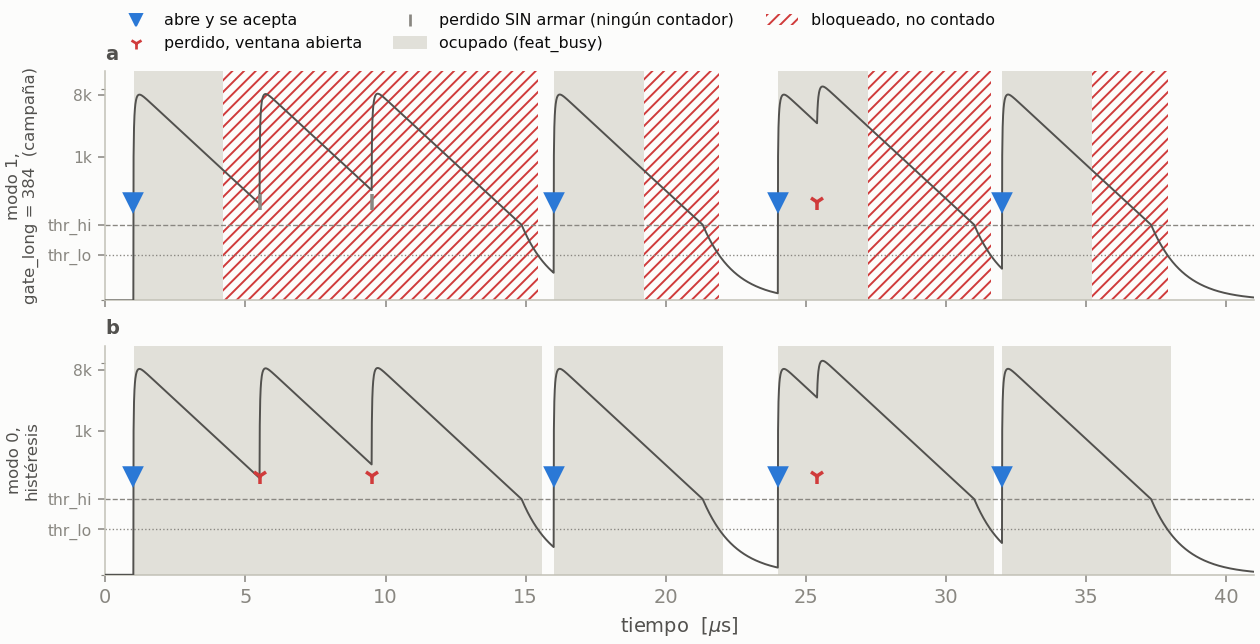
\includegraphics{cap1_politicas_final}
\caption[Criterios de final de evento]{%
Criterios de final de evento sobre el mismo tren de pulsos: (a) política de
ancho fijo, (b) política por histéresis.\label{f:mca-politicas-final}}
\end{figure}

Las marcas rojas señalan una doble falta del sistema ante un pulso que llega con
la ventana abierta. Por un lado, el trigger por nivel no lo detecta, porque la
señal nunca bajó del umbral de re-armado. Por otro, el pulso queda dentro de la
misma ventana: su contribución se suma al estadístico del primero, que pasa a
ser un evento apilado (ver Sec.~\ref{S:mca-pileup}), y con la política por
histéresis además alarga la ventana, porque la señal tarda más en bajar.

Esto obliga a distinguir el \textbf{cierre} de la ventana del
\textbf{re-armado} del disparador. El cierre termina la medición del evento; el
re-armado vuelve a poner disponible el sistema para un nuevo disparo, y en un
disparo por nivel ocurre recién cuando la señal baja de \codigo{thr\_lo}. Con la
ventana por histéresis ambos coinciden, porque ocurren en el mismo nivel; con la
ventana fija no, y entre ambos el sistema queda bloqueado (el intervalo rayado
de la Fig.~\ref{f:mca-politicas-final}). En nuestra implementación ese intervalo
se cuenta por separado (ver Sec.~\refpend{S:implmca-teselado}{Implementación del MCA: teselado del tiempo de adquisición}).

\subsection{\texorpdfstring{\emph{Pileup}}{Pileup}}
\label{S:mca-pileup}

Es la deformación del histograma debida a la \textbf{superposición de pulsos en
la entrada}~\cite{Knoll2010}. Cómo modifica el espectro depende de los
siguientes parámetros:
\begin{enumerate}
  \item La metodología de medición: cómo se abre y se cierra la ventana y qué
    estadístico se calcula (ver Sec.~\ref{S:mca-etapas}).
  \item La distribución de los tiempos entre arribos: para una fuente radiactiva
    los arribos son un proceso de Poisson de tasa $\lambda$,
    $\mathrm{PP}(\lambda)$, y los tiempos entre arribos siguen una exponencial,
    $\mathrm{EXP}(\lambda)$.
  \item La distribución de las alturas de los pulsos superpuestos: las suponemos
    independientes, de modo que el segundo pulso tiene la misma distribución de
    alturas que el primero.
  \item La familia de pulsos (el conformado).
\end{enumerate}

En la Fig.~\ref{f:mca-pileup} comparamos la distribución de alturas ($dN/dH$)
medida para pulsos de dos familias. En la primera fila tenemos un pulso unipolar
con cola positiva, del tipo CR-RC, mientras que en la segunda tenemos un pulso
bipolar, cuya cola es negativa. Cuando el segundo pulso monta sobre la cola del
primero, en el primer caso su altura se sobreestima y aparece un exceso de
cuentas a alturas mayores que la del pico real; en el segundo caso se subestima
y el exceso aparece a alturas menores.

\begin{figure}[H]
\centering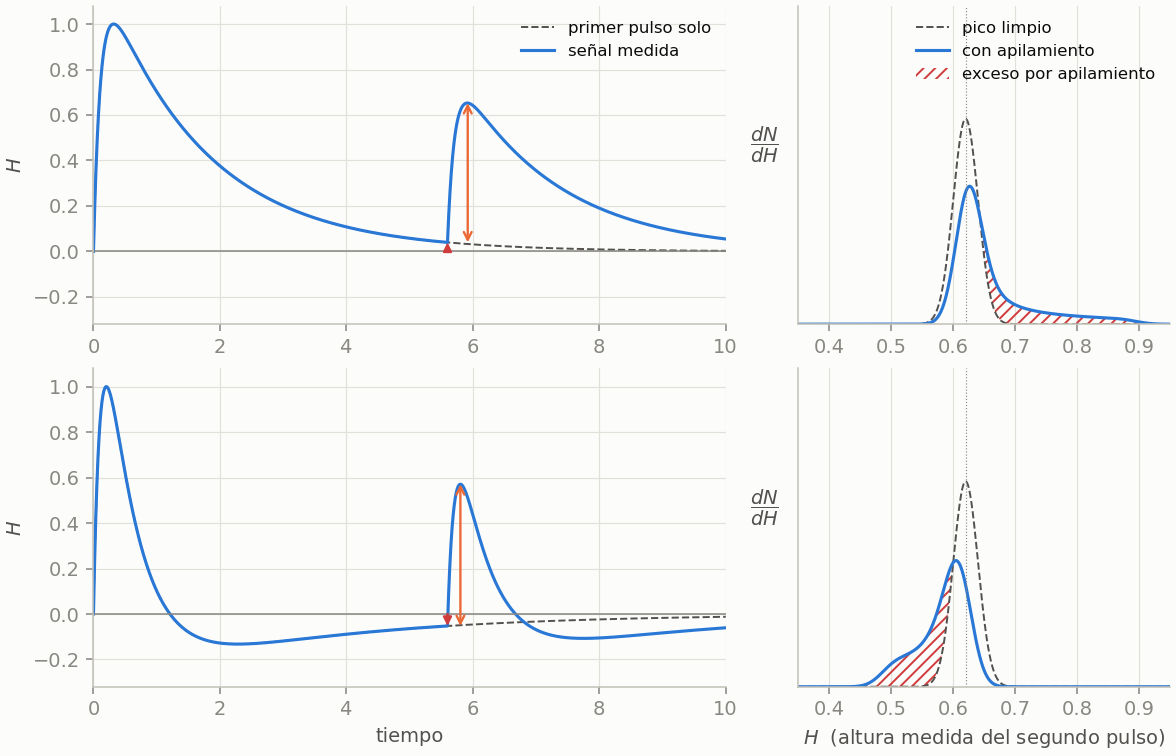
\includegraphics{cap1_pileup}
\caption[Efecto del apilamiento sobre la altura medida]{%
Efecto del apilamiento sobre la altura medida del segundo pulso. Izquierda: la
señal medida y el primer pulso solo; la flecha es la altura medida del segundo.
Derecha: $dN/dH$ del segundo pulso, limpio y con apilamiento; rayado, el exceso
por apilamiento. Arriba, pulso unipolar; abajo, bipolar.\label{f:mca-pileup}}
\end{figure}

Este tipo de distorsión es \emph{compensable} mediante las siguientes dos
técnicas:
\begin{itemize}
  \item Tratamiento teórico o simulado: suponiendo los cuatro parámetros
    anteriores podemos estimar la distribución real. Esta compensación puede
    calcularse de forma teórica o aproximarse mediante Monte-Carlo.
  \item Recuperación en tiempo real: con un sistema de \textbf{seguimiento de
    línea de base}, que estima la amplitud que aportan los pulsos previos y la
    resta. Requiere una implementación en HW; en la
    Sec.~\refpend{S:implmca-linea-base}{Implementación del MCA: recuperación de
    línea de base} se expande sobre este tema.
\end{itemize}

\subsection{Métodos de recuperación de pulso: seguimiento de línea de base}
\label{S:mca-recuperacion-pulso}

Tenemos cuatro posibles formas de tratar el pileup, que se presentan en la
Fig.~\ref{f:mca-metodos-recuperacion}:
\begin{enumerate}
  \item \textbf{No compensar}: calcular el estadístico de la superposición.
  \item \textbf{Descartar}: considerar el evento como no válido.
  \item \textbf{Rescatar un pulso}: inferir un único pulso de la superposición
    presente.
  \item \textbf{Rescatar N pulsos}: inferir hasta N pulsos superpuestos. En la
    Sec.~\refpend{S:implmca-recuperacion}{Implementación del MCA: métodos de
    recuperación del pulso} se desarrolla la complejidad de estas opciones.
\end{enumerate}

\begin{figure}[H]
\centering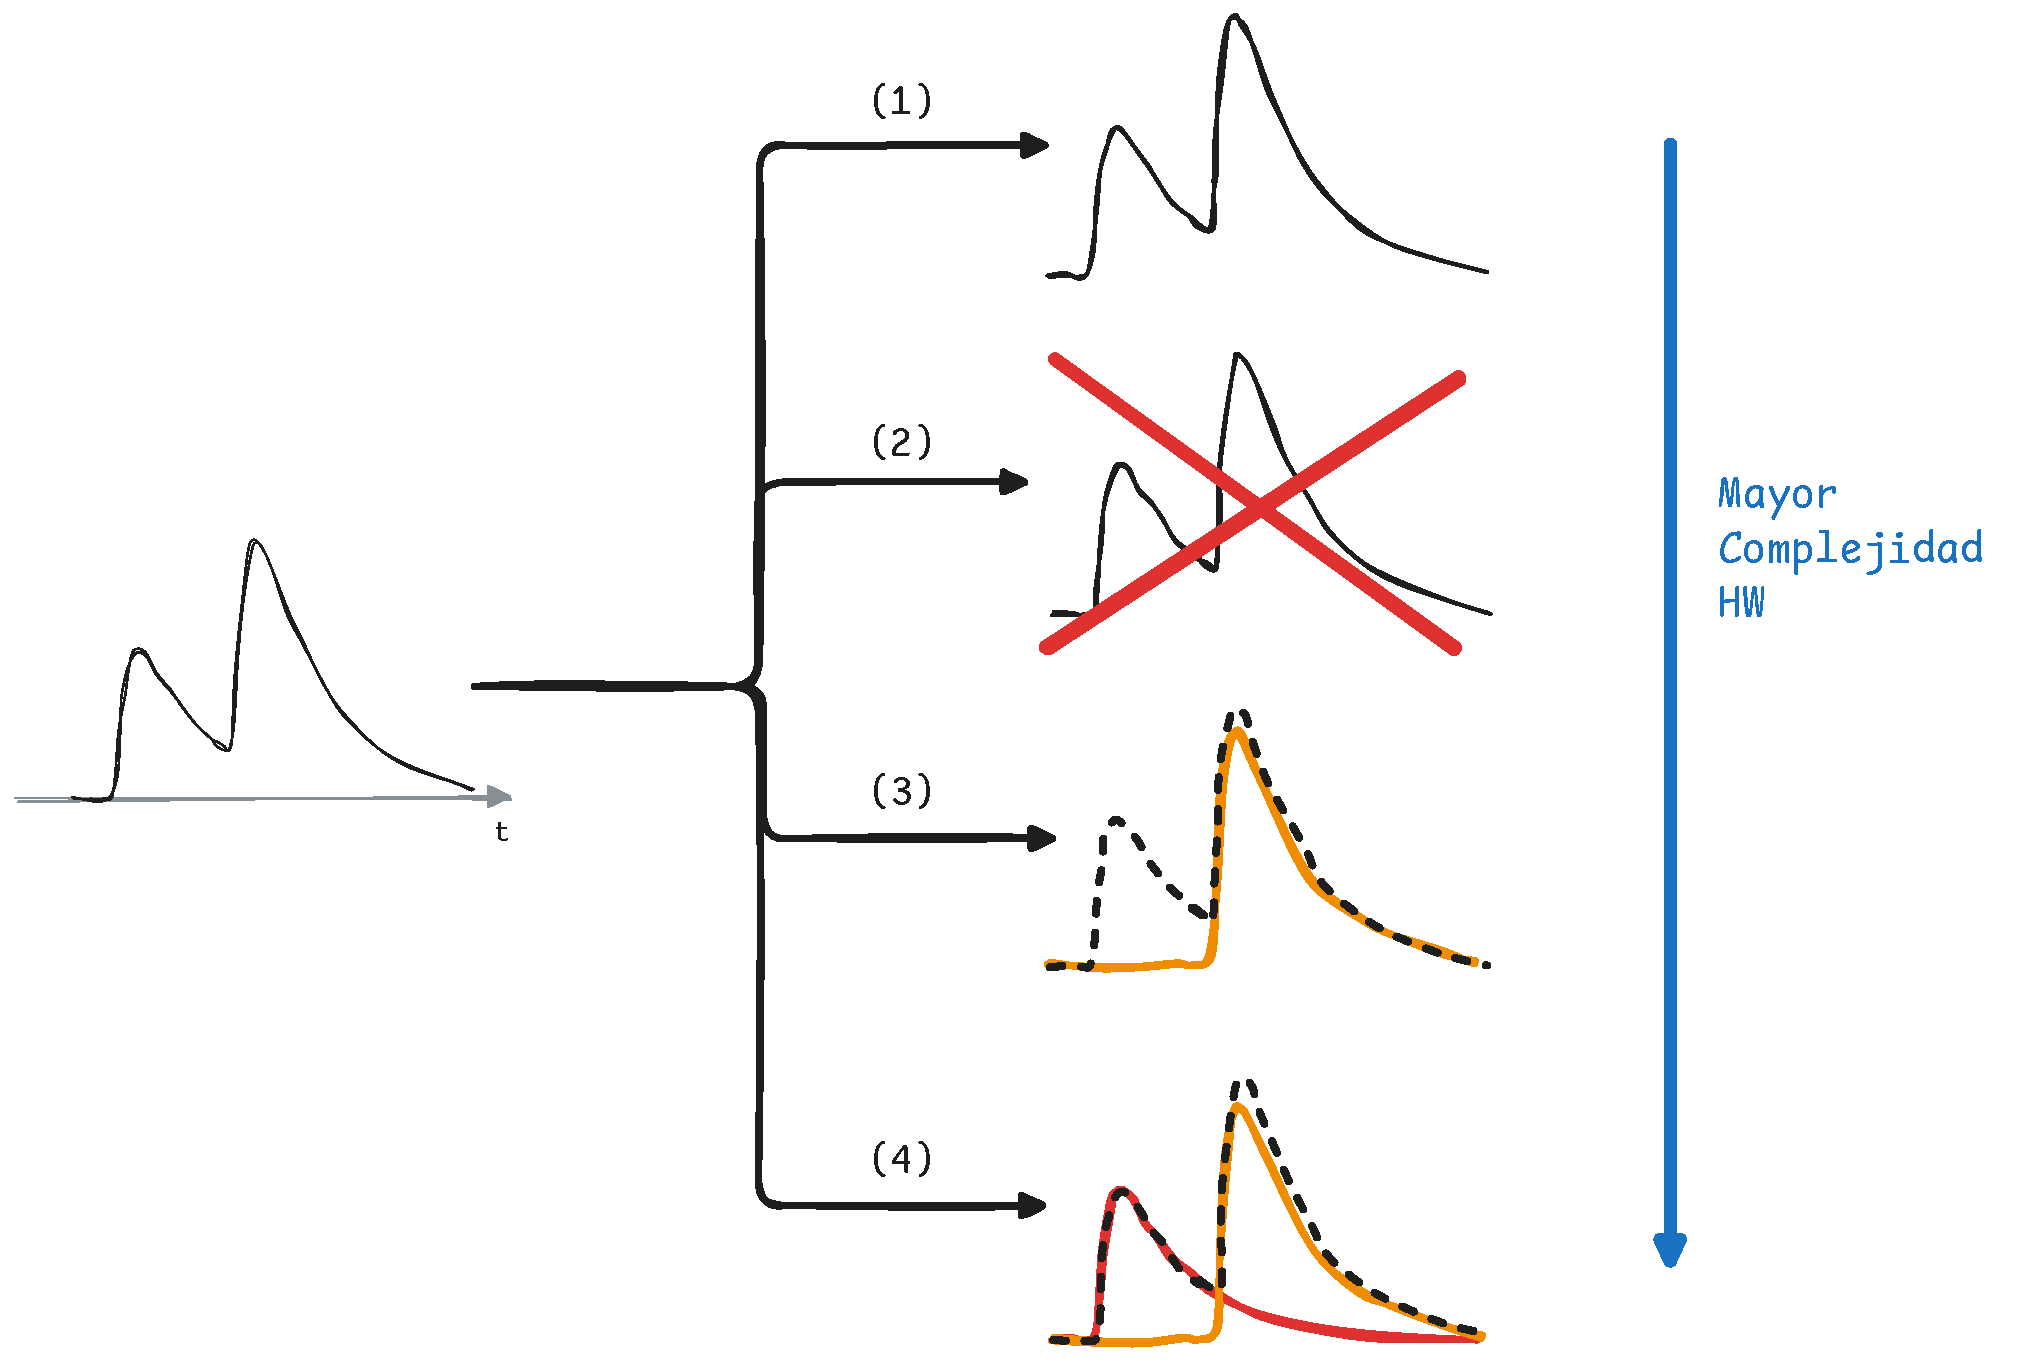
\includegraphics{cap1_metodos_recuperacion}
\caption[Formas de tratar un evento apilado]{%
Las cuatro formas de tratar un evento apilado, ordenadas de menor a mayor
complejidad de HW.\label{f:mca-metodos-recuperacion}}
\end{figure}

La opción de descarte (2) puede ser más que suficiente si los pulsos son
\textbf{independientes en el tiempo}. En ese caso tenemos una reducción en la
cantidad de eventos medidos (y, en consecuencia, en la significancia
estadística), que se resuelve fácilmente aumentando el tiempo de medición.

Esta opción falla cuando los pulsos están \textbf{correlacionados en el tiempo}:
el segundo pulso no llega al azar sino como consecuencia del primero, y
descartar los eventos apilados elimina justamente los de interés. Por ejemplo,
en un detector Cherenkov de agua (\emph{water-Cherenkov
detector})~\cite{Allison2005}, un muón que atraviesa el volumen emite fotones
por efecto Cherenkov a lo largo de su trayectoria. Si el muón se frena y se
detiene dentro del detector, decae en un electrón con una vida media de
$\approx$\qty{2.2}{\micro\second}~\cite{PDG2024}, y el electrón produce un
segundo pulso. Los dos pulsos están correlacionados: su separación sigue una
exponencial de $\approx$\qty{2.2}{\micro\second}, del orden del ancho de los
pulsos conformados, de modo que muchos de esos pares aparecen apilados.

En estos casos conviene rescatar los pulsos, con la tercera o la cuarta opción,
que tienen un criterio de corrección:
\begin{itemize}
  \item La tercera necesita una prioridad para decidir qué pulso rescata, pero
    tiene la ventaja de que \textbf{cada evento se asocia con un único cálculo
    de estadístico}, por lo que es más simple de implementar.
  \item La cuarta requiere poder procesar múltiples pulsos por evento.
    \textbf{Requiere implementar una cola de procesamiento dentro del sistema};
    los detalles se encuentran en la
    Sec.~\refpend{S:implmca-recuperacion}{Implementación del MCA: métodos de
    recuperación del pulso}.
\end{itemize}

\subsection{\texorpdfstring{\emph{Amplitude walk}}{Amplitude walk}}
\label{S:mca-amplitude-walk}

Es la \textbf{diferencia temporal en el disparo} de eventos de una misma familia
de pulsos debida a la diferencia en su amplitud máxima~\cite{Knoll2010}. En la
Fig.~\ref{f:mca-amplitude-walk} se presentan tres pulsos de la misma forma, con
igual tiempo de subida $t_s$ y de bajada $t_b$, que llegan exactamente al mismo
tiempo pero tienen distinta amplitud.

\begin{figure}[H]
\centering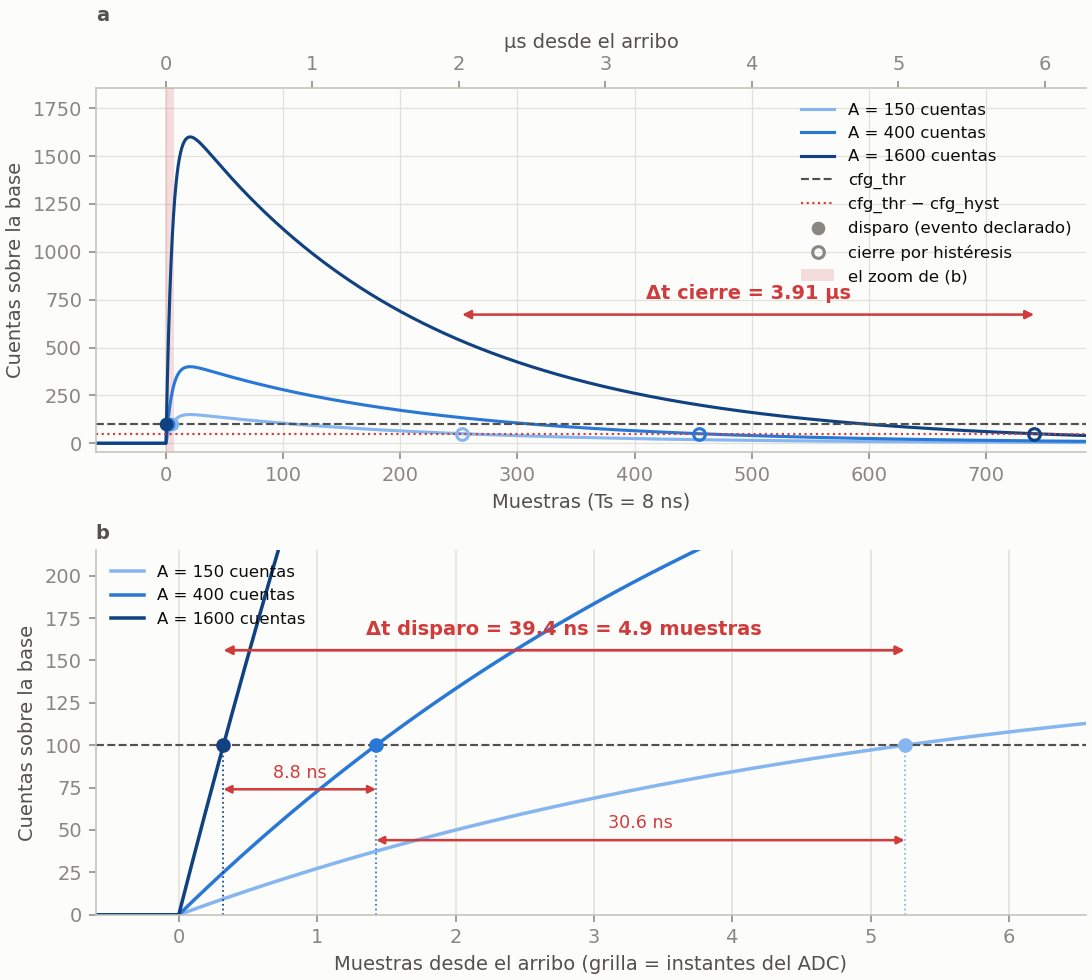
\includegraphics{cap1_amplitude_walk}
\caption[\emph{Amplitude walk} para tres pulsos de la misma familia]{%
(a) \emph{Amplitude walk} para tres pulsos de la misma familia que llegan a la
vez, con el disparo y el cierre por histéresis de cada uno. (b) Detalle de la
diferencia temporal de disparo entre los tres pulsos.\label{f:mca-amplitude-walk}}
\end{figure}

Sin embargo, la detección del pulso de 1600~ADU ocurre \qty{8.8}{\nano\second}
antes que la del de 400~ADU, y \qty{39.4}{\nano\second} antes que la del de
150~ADU: el pulso más grande cruza el umbral primero porque sube más rápido.

De esta forma tenemos una distribución de largos de la \textbf{ventana de tiempo
previa al disparo}: la porción de la subida que queda antes del disparo depende
de la amplitud. Generalmente nos importa su valor máximo, que corresponde a los
pulsos más chicos. Según el conformado esto puede no ser un problema; es peor
para conformados con tiempos de subida lentos, especialmente para el CR-RC$^4$.
El walk también corre el cierre por histéresis, y mucho más, porque ese cruce
ocurre sobre la cola exponencial: en la Fig.~\ref{f:mca-amplitude-walk}(a) los
cierres de los tres pulsos se separan \qty{3.91}{\micro\second}.

En nuestra implementación se decidió que la ventana de tiempo previa al disparo
sea fija: la señal se retrasa una cantidad configurable de ciclos antes de
entrar a la ventana, de modo que el pie del pulso ya esté adentro cuando llega
el disparo. Para la altura máxima es una buena decisión, porque la subida no se
descarta y el ápice queda siempre dentro de la ventana. Para los estadísticos
que integran la subida, como la carga o el factor de forma, la porción de la
ventana previa que cae antes del pie del pulso depende de la amplitud: si no se
resta la línea de base, esa porción suma a la carga un término que varía con la
amplitud, y si el retardo no alcanza a cubrir el walk de los pulsos más chicos,
a ellos se les pierde parte de la subida. En ambos casos es una no linealidad
concentrada cerca del umbral, y por eso estos estadísticos se calculan sobre la
señal con la línea de base restada (ver
Sec.~\refpend{S:implmca-linea-base}{Implementación del MCA: recuperación de
línea de base}).

%%%%%%%%%%%%%%%%%%%%%%%%%%%%%%%%%%%%%%%%%%%%%%%%%%%%%%%%%%%%%%%%%%%%%%%%%%%%%%%%
\section{Tiempo muerto y tiempo vivo}
\label{S:mca-tiempo-muerto}

Inicialmente definimos el tiempo muerto como \textbf{el tiempo en el cual el
sistema no puede procesar un nuevo evento de la forma deseada}; el tiempo vivo
es su complemento. Sus causas incluyen limitaciones en cada una de las secciones
del sistema. Reducirlo es la razón principal de la existencia del MCA: como
procesa cada evento en el hardware y solo transfiere el histograma, su tiempo
muerto es un orden de magnitud menor que el de la captura de trazas con el
módulo de osciloscopio (OSC). En la Sec.~\ref{S:intro-hw-back-pressure}
describimos cómo \textbf{medir} y diseñar un sistema para reducir al máximo el
tiempo muerto de medición.

\subsection{Modelos fundamentales de tiempo muerto}
\label{S:mca-modelos-tiempo-muerto}

Por el tiempo muerto, la tasa registrada $m$ es menor que la tasa real de
eventos $n$. Para corregirla necesitamos un modelo que vincule ambas, y todo
modelo depende del tiempo muerto $\tau$. En esta sección presentamos los dos
modelos más sencillos y mostramos por qué \textbf{necesitamos determinar $\tau$
con precisión}: la corrección amplifica cualquier error en $\tau$, y la
amplificación crece con la tasa.

Ambos modelos describen el comportamiento del sistema frente a eventos
sucesivos separados un tiempo $\Delta T$. Uno se denomina
\textbf{paralizable}, porque cada vez que llega un evento la ventana de tiempo
muerto se reinicia, aunque ese evento no se registre. En el \textbf{no
paralizable}, en cambio, la ventana de tiempo muerto no se reinicia por la
llegada de nuevos eventos: lo que llega durante ella se pierde sin extenderla.
En la Fig.~\ref{f:mca-tren-rho05} se presenta el mismo tren de arribos para
ambos modelos.

\begin{figure}[H]
\centering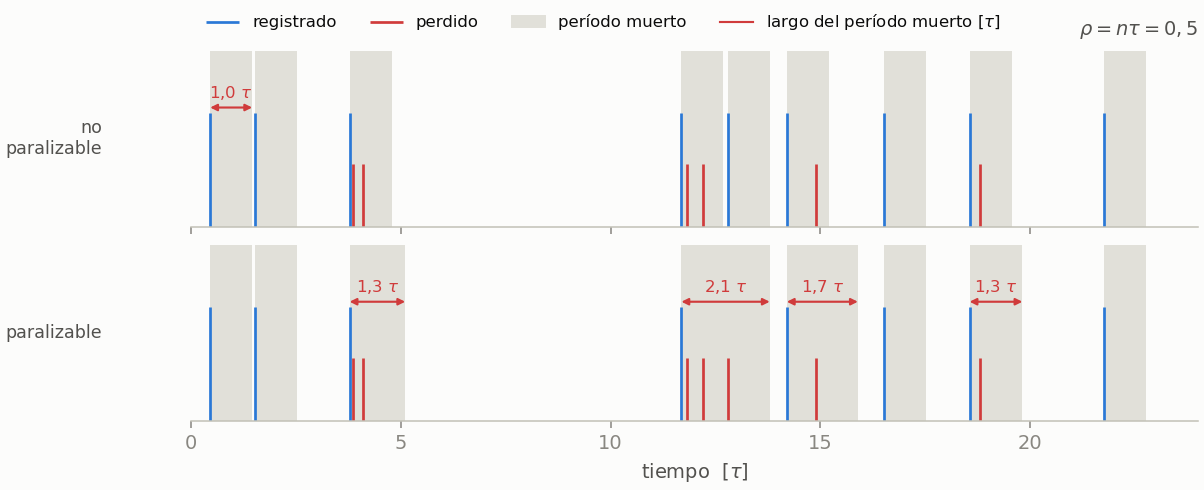
\includegraphics{cap1_tren_rho05}
\caption[Un tren de arribos de Poisson visto por los dos modelos de tiempo
muerto]{%
Un mismo tren de arribos de Poisson con $\rho = n\tau = 0.5$ visto por los dos
modelos. En el no paralizable cada período muerto dura $\tau$; en el
paralizable los arribos perdidos lo extienden.\label{f:mca-tren-rho05}}
\end{figure}

Para cada uno de estos modelos podemos calcular los parámetros importantes, como
la fracción de tiempo vivo, la fracción de eventos aceptados, el largo promedio
de la ventana muerta y, el más importante de todos, la \textbf{tasa registrada
en función de la tasa incidente}. En la Tabla~\ref{t:mca-tiempo-muerto} se
presentan las relaciones fundamentales de los dos modelos para arribos de
Poisson; su deducción se encuentra en Knoll~\citecap{Knoll2010}{4}, y una
revisión de sus variantes, en Müller~\cite{Muller1973}.

\begin{table}[H]
\centering
\caption[Modelos de tiempo muerto no paralizable y paralizable]{%
Relaciones fundamentales de los modelos no paralizable y paralizable para
arribos de Poisson de tasa $n$; $W$ es la función de
Lambert~\cite{Corless1996}.\label{t:mca-tiempo-muerto}}
\renewcommand{\arraystretch}{2.1}
\begin{tabular}{|l|c|c|}
\hline
\encabezado & \textbf{No paralizable} (tipo I) & \textbf{Paralizable} (tipo II) \\ \hline
Tasa registrada           & $m = \dfrac{n}{1+n\tau}$
                          & $m = n\,e^{-n\tau}$ \\ \hline
Tasa real despejada       & $\hat n = \dfrac{m}{1-m\tau}$
                          & $\hat n = -\dfrac{W(-m\tau)}{\tau}$ \\ \hline
Fracción perdida          & $1-\dfrac{m}{n} = \dfrac{n\tau}{1+n\tau}$
                          & $1-\dfrac{m}{n} = 1-e^{-n\tau}$ \\ \hline
Fracción de tiempo muerto & $m\tau = \dfrac{n\tau}{1+n\tau}$
                          & $1-e^{-n\tau}$ \\ \hline
Límite $n\tau\ll 1$       & $m \simeq n\,(1-n\tau)$
                          & $m \simeq n\,(1-n\tau)$ \\ \hline
Límite $n\to\infty$       & $m \to 1/\tau$
                          & $m \to 0$ \\ \hline
Máximo                    & no tiene, es monótona
                          & $m_{\max} = \dfrac{1}{e\,\tau}$ en $n = 1/\tau$ \\ \hline
\end{tabular}
\end{table}

En la Fig.~\ref{f:mca-tasa-registrada} representamos la \textbf{tasa medida
normalizada} $m\tau$ \textbf{en función de la tasa incidente normalizada}
$n\tau$, en el estado estacionario, para ambos modelos. El producto
$\rho = n\tau$ es la cantidad promedio de eventos incidentes durante una ventana
de tiempo muerto, y es el único parámetro del que dependen las curvas. A tasas
bajas, $n\tau \ll 1$, los dos modelos coinciden y $m \simeq n$. A medida que
$n\tau$ se acerca a 1 se separan, y en $n\tau = 1$ ya se registra a lo sumo la
mitad de los eventos ($m\tau = 1/2$ en el no paralizable y
$m\tau = 1/e \approx 0.37$ en el paralizable).

\begin{figure}[H]
\centering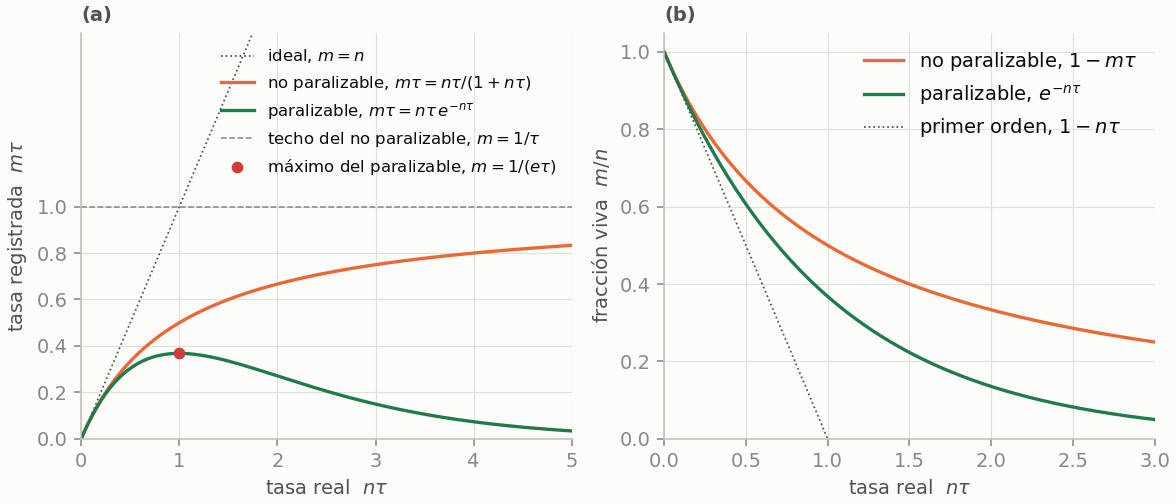
\includegraphics{cap1_tasa_registrada}
\caption[Tasa registrada contra tasa incidente]{%
(a) Tasa registrada contra tasa incidente, ambas normalizadas por $\tau$, para
los dos modelos y la diagonal ideal. (b) La fracción de tiempo vivo de la que
salen las dos fórmulas.\label{f:mca-tasa-registrada}}
\end{figure}

La implicancia es doble. Por un lado, la \textbf{cantidad de cuentas medidas en
un tiempo $T$ no es lineal con la tasa incidente}:
\begin{equation}
  N_T = m\,T = \frac{n\,T}{1+n\tau}\quad\text{(no paralizable)},\qquad
  N_T = n\,T\,e^{-n\tau}\quad\text{(paralizable)}
  \label{e:mca-cuentas}
\end{equation}
En el caso paralizable la relación ni siquiera es monótona: $N_T$ alcanza un
máximo $T/(e\tau)$ en $n = 1/\tau$ y decrece después, de modo que aumentar la
actividad de la fuente \textbf{reduce} la estadística disponible.

Por otro lado, la tasa real no se mide: se \textbf{estima} invirtiendo el
modelo, $\hat n(m, \tau)$, y esa estimación hereda los errores de las dos
magnitudes que entran en ella. El error en la tasa medida $m$ es estadístico y
se reduce midiendo más tiempo; el error en $\tau$ depende de qué tan bien
conozcamos el sistema. Para ver cuánto pesa cada uno propagamos a primer orden:
\begin{equation}
  \delta \hat n = \frac{\partial \hat n}{\partial m}\,\delta m
                + \frac{\partial \hat n}{\partial \tau}\,\delta \tau
  \label{e:mca-propagacion}
\end{equation}
En el caso no paralizable la estimación es explícita, $\hat n = m/(1-m\tau)$, y
las dos derivadas parciales, los \textbf{coeficientes de
sensibilidad}~\cite{GUM2008} de la medición, se calculan de forma directa:
\begin{equation}
  \frac{\partial \hat n}{\partial m} = \frac{1}{(1-m\tau)^2}, \qquad
  \frac{\partial \hat n}{\partial \tau} = \frac{m^2}{(1-m\tau)^2}
  \label{e:mca-sensibilidad-np}
\end{equation}
Pasamos a errores relativos, que son los que entrega la estadística de conteo y
los que tiene sentido reportar, dividiendo por $\hat n$ y usando
$n\tau = m\tau/(1-m\tau)$:
\begin{equation}
  \begin{split}
  \frac{\delta \hat n}{\hat n}
    &= \frac{1}{1-m\tau}\,\frac{\delta m}{m}
     + \frac{m\tau}{1-m\tau}\,\frac{\delta \tau}{\tau} \\
    &= (1+n\tau)\,\frac{\delta m}{m} + n\tau\,\frac{\delta \tau}{\tau}
  \end{split}
  \label{e:mca-relativo-np}
\end{equation}
Los dos coeficientes difieren exactamente en una unidad.

El caso paralizable no admite un despeje elemental, pero tampoco lo necesita:
basta con diferenciar el modelo directo $m = n\,e^{-n\tau}$ de forma implícita y
usar $e^{n\tau} = n/m$ para simplificar el primer término:
\begin{equation}
  \begin{gathered}
  \delta m = e^{-n\tau}\Big[(1-n\tau)\,\delta n - n^2\,\delta \tau\Big] \\
  \Longrightarrow\qquad
  \frac{\delta n}{n} = \frac{1}{1-n\tau}\,\frac{\delta m}{m}
                     + \frac{n\tau}{1-n\tau}\,\frac{\delta \tau}{\tau}
  \end{gathered}
  \label{e:mca-relativo-p}
\end{equation}
De nuevo, los dos coeficientes difieren en una unidad.

No es una coincidencia. Escrita en las cantidades adimensionales $m\tau$ y
$n\tau$, toda calibración es una función $n\tau = g(m\tau)$ sin parámetros
libres, y la estimación es $\hat n = g(m\tau)/\tau$. Aplicando la regla del
producto y normalizando cada coeficiente de sensibilidad:
\begin{equation}
  \begin{gathered}
  \frac{m}{\hat n}\frac{\partial \hat n}{\partial m}
    = \frac{m\tau\,g'(m\tau)}{g(m\tau)} \equiv E, \\
  \frac{\tau}{\hat n}\frac{\partial \hat n}{\partial \tau}
    = \frac{m\tau\,g'(m\tau)}{g(m\tau)} - 1 = E-1
  \end{gathered}
  \label{e:mca-E}
\end{equation}
Llamamos a $E$ el \textbf{término de amplificación de error}. Es la pendiente de
la curva de calibración en escala logarítmica,
$E = d\ln(n\tau)/d\ln(m\tau)$: la corrección amplifica los errores exactamente
en la medida en que esa curva se aplana. Como $m$ y $\tau$ son magnitudes
independientes, sus contribuciones se combinan en cuadratura según la ley de
propagación de incertidumbres~\cite{GUM2008}:
\begin{equation}
  \left(\frac{\delta \hat n}{\hat n}\right)^{2}
    = E^{2}\left(\frac{\delta m}{m}\right)^{2}
    + (E-1)^{2}\left(\frac{\delta \tau}{\tau}\right)^{2}
  \label{e:mca-cuadratura}
\end{equation}
con
\begin{equation}
  E = \frac{1}{1-m\tau} = 1+n\tau \quad\text{(no paralizable)}, \qquad
  E = \frac{1}{1-n\tau} \quad\text{(paralizable)}
  \label{e:mca-E-modelos}
\end{equation}

El coeficiente que pesa el error en $\tau$, $E-1$, es el que motiva esta
sección. Vale $n\tau$ en el modelo no paralizable y $n\tau/(1-n\tau)$ en el
paralizable: se anula a tasa baja, donde la corrección misma es chica, y crece
con la tasa. A $n\tau = 0.5$, un error del \qty{1}{\percent} en $\tau$ se
convierte en un error de \qty{0.5}{\percent} en la tasa corregida en el modelo
no paralizable y de \qty{1}{\percent} en el paralizable; a $n\tau = 0.9$, en
\qty{0.9}{\percent} y \qty{9}{\percent}, respectivamente. Además, este error es
\textbf{sistemático}: a diferencia del de $m$, no se reduce aumentando el tiempo
de medición. La incerteza en $\tau$ fija entonces un piso a la exactitud de la
tasa corregida y, con él, la tasa máxima a la que podemos trabajar con una
exactitud dada. Por eso \textbf{necesitamos determinar $\tau$ con precisión}, y
no tomarlo de un valor nominal: un $\tau$ mal determinado produce variaciones
grandes en las tasas corregidas, justamente en el régimen de tasas altas, que es
donde la corrección más importa.

Si graficamos ambos coeficientes obtenemos la
Fig.~\ref{f:mca-amplificacion}: el panel (a) muestra $E$, el factor que pesa el
error en la tasa medida, y el (b) muestra $E-1$, el que pesa el error en el
tiempo muerto, ambos contra $\rho = n\tau$. En el modelo no paralizable la
pendiente de la calibración decae suavemente y $E$ crece de forma lineal con la
tasa. En el paralizable la calibración se vuelve horizontal en $\rho = 1$ y $E$
diverge, porque allí ningún valor medido distingue tasas incidentes vecinas.
Para $\rho > 1$ el coeficiente del modelo paralizable cambia de signo, porque se
está en la rama descendente de la curva; la figura grafica su valor absoluto,
así que su caída pasado $\rho = 1$ no indica que la corrección mejore.

\begin{figure}[H]
\centering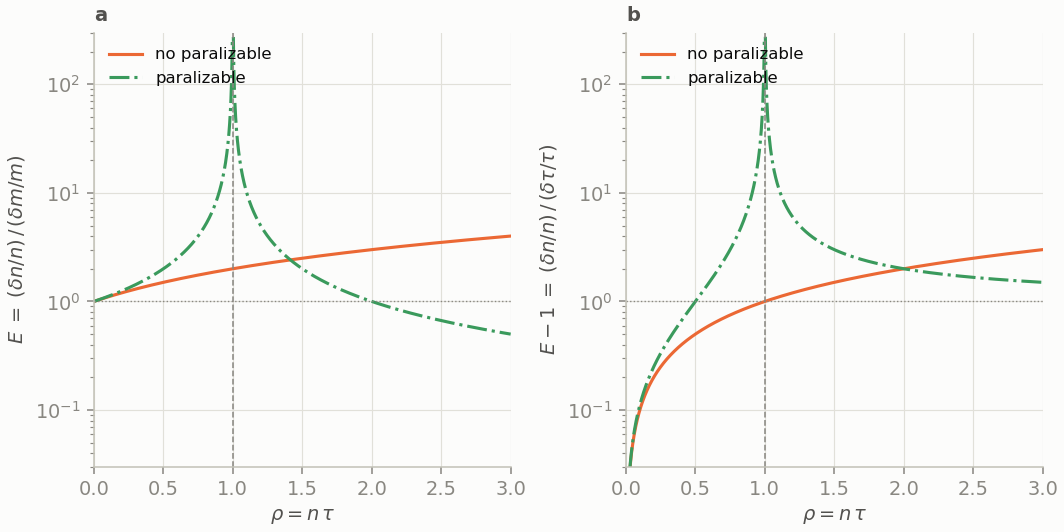
\includegraphics{cap1_amplificacion_correccion}
\caption[Amplificación de error de la corrección de tasa]{%
Amplificación de error de la corrección de tasa en función de $\rho = n\tau$:
(a) $E$, que pesa el error relativo de la tasa medida; (b) $E-1$, que pesa el
error relativo del tiempo muerto.\label{f:mca-amplificacion}}
\end{figure}

Para la versión paralizable hay además un problema cualitativo: al no ser
monótona, a una misma tasa medida le corresponden \textbf{dos} tasas incidentes
posibles, una a cada lado de $n = 1/\tau$. Sin una idea previa del rango de
tasas o alguna medición auxiliar, no es posible decidir cuál de las dos
correcciones es la correcta.

\begin{destacado}
Es así que nos propusimos que nuestro sistema tenga la capacidad de
\textbf{reportar la distribución del tiempo muerto} y la cantidad de
\textbf{eventos rechazados}, de modo de medir el tiempo muerto en cada
adquisición en lugar de suponerlo, y de poder analizar posteriormente qué tan
válidos son los resultados obtenidos y cuál de los dos modelos aplica a nuestro
sistema.
\end{destacado}

Esto es necesario porque cuál de los modelos aplica mejor \textbf{depende de los
parámetros elegidos}. En la Fig.~\ref{f:mca-politicas-final}(b), por ejemplo, la
llegada de nuevos pulsos alarga la ventana, porque esta termina recién cuando la
señal decae hasta el nivel de relajación: es un comportamiento paralizable. Lo
mismo ocurre con la ventana fija de (a), porque el disparador por nivel no se
re-arma mientras la cola siga por encima del umbral, y cada pulso que llega en
ese lapso la mantiene arriba.

Un caso típico en el que ninguno de los dos modelos aplica es el ensayo con una
fuente periódica de laboratorio, como un generador de pulsos, en la que la
separación entre pulsos es constante. Si el período es mayor que $\tau$, cada
pulso encuentra al sistema libre y no se pierde ninguno; con arribos de Poisson,
en cambio, se pierde una fracción $\approx n\tau$ a cualquier tasa, porque los
arribos se agrupan. Una eficiencia medida con un generador periódico es una
propiedad del estímulo y no del equipo, y no puede trasladarse a una fuente
radiactiva. Por eso, para caracterizar el tiempo muerto usamos también trenes
de pulsos con arribos de Poisson.

%%%%%%%%%%%%%%%%%%%%%%%%%%%%%%%%%%%%%%%%%%%%%%%%%%%%%%%%%%%%%%%%%%%%%%%%%%%%%%%%
\section{Características de mérito del sistema}
\label{S:mca-merito}

Con estas caracterizamos la desviación, RMS o máxima, de la respuesta del
sistema respecto de la esperada. La caracterización experimental consiste en
inyectar una secuencia de pulsos conocida y analizar la distribución obtenida.
En la Fig.~\ref{f:mca-merito} se presentan los tres parámetros más importantes
(Knoll~\citecap{Knoll2010}{18}): la resolución FWHM, la no linealidad integral
(INL) y la no linealidad diferencial (DNL). Las tres son independientes y
arruinan cosas distintas: la INL corre el pico, la DNL lo deforma y la
resolución finita lo ensancha.

\begin{figure}[H]
\centering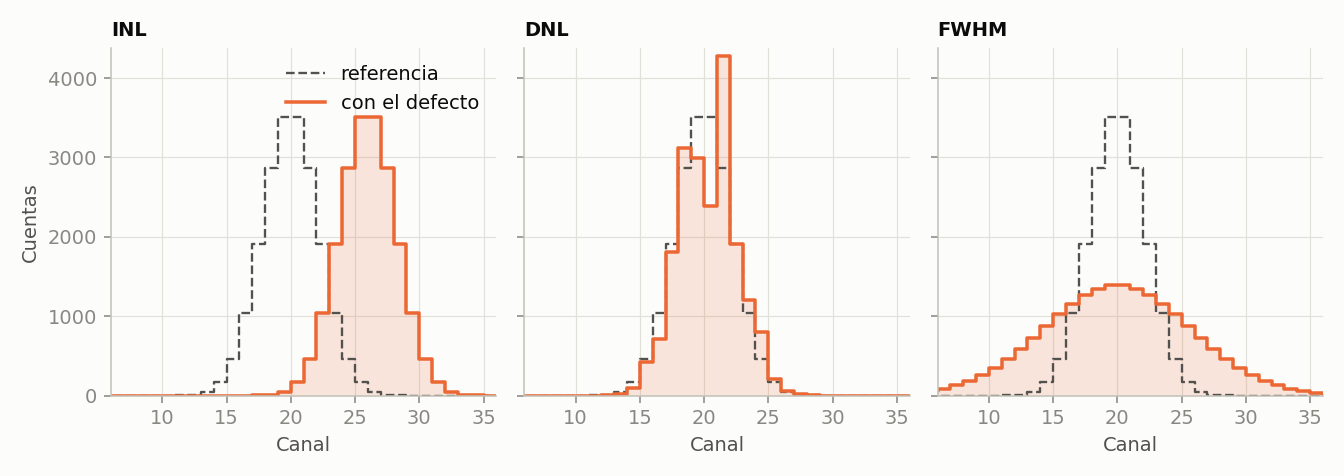
\includegraphics{cap1_tres_metricas}
\caption[Figuras de mérito de un MCA: FWHM, INL y DNL]{%
El mismo pico de referencia (línea de trazos) visto con cada defecto por
separado. Datos sintéticos.\label{f:mca-merito}}
\end{figure}

\subsection{Resolución FWHM}
\label{S:mca-fwhm}

Es el \textbf{ancho del pico a media altura}, de ahí su nombre: \emph{full width
at half maximum} (FWHM). Normalmente se lo expresa como porcentaje de la altura
de su centroide $H_0$, $R = \mathrm{FWHM}/H_0$. Pulsos idénticos caerían todos
en un mismo canal, así que el ancho que se mide es ensanchamiento: ruido de la
cadena, cuantización y jitter del estimador de amplitud. Es el piso del sistema
y la única de las tres métricas que no se compensa por software, porque el
ensanchamiento es aleatorio. Cuando el pico se ensancha, dos líneas cercanas
dejan de separarse.

\subsection{No linealidad integral (INL)}
\label{S:mca-inl}

El amplificador ideal consiste en una ganancia lineal $G$, de forma que la
amplitud medida ideal sería $\hat A_\text{ideal} = G A$. Las no idealidades
generalmente se tienen en cuenta con dos parámetros: el offset del cero $A_0$ y
el residuo a lo largo de la curva de amplificación,
\begin{equation}
  \hat A = G \cdot (A-A_0) + \text{INL}(A-A_0)
  \label{e:mca-inl}
\end{equation}
La INL mide cuánto se aparta la relación real entre amplitud y canal de la
\textbf{recta ideal}~\cite{IEEE1241}. Es una función $\text{INL}(A)$, pero
normalmente se la describe por su valor máximo,
$\text{INL} = \max_A |\text{INL}(A)|$.

En el panel INL de la Fig.~\ref{f:mca-merito} se representa un ejemplo con
$A_0 = 0$, en el que la expresión se simplifica a
$\hat A = G \cdot A + \text{INL}(A)$: la forma del pico queda intacta, pero el
pico está donde no va. En la práctica se ajusta una recta a los centroides
medidos para varias amplitudes, y el residuo del ajuste es $\text{INL}(A)$. Se
la calcula con la siguiente expresión
\begin{equation}
  \text{INL} = \frac{\max|\text{residuo}|}{\text{canal}_{\max} - \text{canal}_{\min}}
  \label{e:mca-inl-max}
\end{equation}
y generalmente se la expresa en porcentaje del rango barrido o del fondo de
escala. Como es un error sistemático, la INL se puede compensar con una
calibración. La curva medida en nuestro sistema se presenta en la
Sec.~\ref{S:res-inl-trapecio}.

\subsection{No linealidad diferencial (DNL)}
\label{S:mca-dnl}

Es la \textbf{variación} del \textbf{ancho de cada canal respecto del
promedio}~\cite{IEEE1241},
$\text{DNL}_i = \Delta H_i / \overline{\Delta H} - 1$. Se mide llenando el
espectro con amplitudes uniformemente distribuidas, por ejemplo con un
generador de amplitud deslizante: si todos los canales fueran iguales recibirían
la misma cantidad de cuentas, así que la desviación relativa de las cuentas
\emph{es} la DNL.

Un canal más ancho junta más cuentas y \textbf{crea estructura que no está en la
señal}: deforma los picos, sesga el área y el centroide, y en el peor caso
genera picos falsos. Cuando es periódica (típico de los ADC, en las transiciones
de bits) produce un rizado regular en todo el espectro.

\subsection{Resolución de par de pulsos}
\label{S:mca-par-pulsos}

Es la capacidad de un sistema de \textbf{disparo} de distinguir dos pulsos
superpuestos separados un tiempo $\Delta t$ variable; se la caracteriza con la
menor separación a la que el sistema dispara dos veces. Una propiedad distinta
es la capacidad de recuperar los estadísticos de los pulsos originales a partir
de su superposición; para ello se refiere a la
Sec.~\refpend{S:implmca-linea-base}{Implementación del MCA: recuperación de
línea de base}.

\subsection{Selección del tipo de bineado}
\label{S:mca-bineado}

Podemos configurar el módulo de forma que el indexado de la memoria de
acumulación tenga \textbf{dos índices en lugar de uno solo}, con lo que el
histograma medido se vuelve 2D. Esto nos da dos opciones:
\begin{enumerate}
  \item Histograma 1D de $2^N$ divisiones.
  \item Histograma 2D de $2^{N_1} \times 2^{N_2}$ divisiones.
\end{enumerate}

Como empleamos división uniforme en ambos casos, la demanda de memoria en el
caso 2D escala con el producto de las divisiones, $2^{N_1+N_2}$. Con la misma
memoria que un histograma 1D de $2^N$ canales, el 2D reparte los bits entre los
dos ejes, $N_1 + N_2 = N$, y cada eje queda con mucha menos resolución.

Algunas aplicaciones del MCA 2D \emph{intracanal}, es decir, en el que ambas
\textbf{features son del mismo evento}, se presentan en el
Apéndice~\ref{S:ap-mca2d}. En la Fig.~\ref{f:mca-2d} se presenta un ejemplo de
histograma de dos variables para la \textbf{identificación
$\alpha/\beta/\gamma$}, en el que se grafica la altura máxima contra un factor
de forma del pulso para separar las partículas $\alpha$ de las $\beta/\gamma$.

\begin{figure}[H]
\centering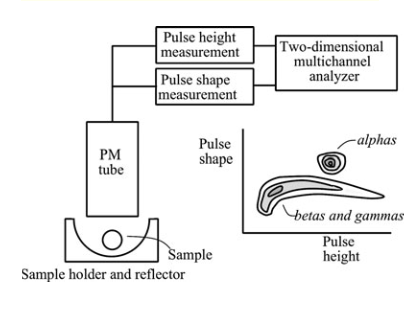
\includegraphics[width=0.6\linewidth]{cap1_mca2d_knoll}
\caption[Identificación $\alpha/\beta/\gamma$ con un histograma de dos
variables]{%
Identificación $\alpha/\beta/\gamma$ con un histograma de dos variables.
Extraída de Knoll~\cite{Knoll2010}.\label{f:mca-2d}}
\end{figure}

Existen también MCA 2D cuyos ejes trabajan sobre \textbf{eventos de diferentes
canales}. En particular, permiten un análisis de coincidencias y
anticoincidencias~\cite{Knoll2010}, en el que el disparo de un evento requiere
varias condiciones mutuas. El caso más sencillo es la coincidencia: que dos
canales disparen dentro de una ventana de tiempo $\Delta T$ dada. En la
anticoincidencia, en cambio, se requiere que un canal en particular dispare y
que otro \textbf{no} lo haga dentro de la ventana.

% Bibliografía de este capítulo. Va al final del archivo, siempre.
\bibliografiacapitulo

%%% Local Variables:
%%% mode: latex
%%% TeX-master: "template"
%%% End:
